% Options for packages loaded elsewhere
\PassOptionsToPackage{unicode}{hyperref}
\PassOptionsToPackage{hyphens}{url}
\PassOptionsToPackage{dvipsnames,svgnames,x11names}{xcolor}
%
\documentclass[
  12pt,
]{article}
\title{\hfill\break
\hfill\break
\hfill\break
\vspace{1cm}Customer dropout membership\footnote{Corresponding address: \href{mailto:sobreiro@esdrm.ipsantarem.pt}{\nolinkurl{sobreiro@esdrm.ipsantarem.pt}}. Quality of Life Research Centre, Polytechnic Institute of Santarém, Portugal}\vspace{0.5cm}}
\author{Pedro Sobreiro, Javier Berrocal, Domingos Martinho, José Garcia Alonso\\
\strut \\
Extremadura University\\}
\date{\hfill\break
\hfill\break
9 outubro, 2021\\
\strut \\}

\usepackage{amsmath,amssymb}
\usepackage{lmodern}
\usepackage{setspace}
\usepackage{iftex}
\ifPDFTeX
  \usepackage[T1]{fontenc}
  \usepackage[utf8]{inputenc}
  \usepackage{textcomp} % provide euro and other symbols
\else % if luatex or xetex
  \usepackage{unicode-math}
  \defaultfontfeatures{Scale=MatchLowercase}
  \defaultfontfeatures[\rmfamily]{Ligatures=TeX,Scale=1}
  \setmainfont[]{Times New Roman}
  \setsansfont[]{Times New Roman}
\fi
% Use upquote if available, for straight quotes in verbatim environments
\IfFileExists{upquote.sty}{\usepackage{upquote}}{}
\IfFileExists{microtype.sty}{% use microtype if available
  \usepackage[]{microtype}
  \UseMicrotypeSet[protrusion]{basicmath} % disable protrusion for tt fonts
}{}
\makeatletter
\@ifundefined{KOMAClassName}{% if non-KOMA class
  \IfFileExists{parskip.sty}{%
    \usepackage{parskip}
  }{% else
    \setlength{\parindent}{0pt}
    \setlength{\parskip}{6pt plus 2pt minus 1pt}}
}{% if KOMA class
  \KOMAoptions{parskip=half}}
\makeatother
\usepackage{xcolor}
\IfFileExists{xurl.sty}{\usepackage{xurl}}{} % add URL line breaks if available
\IfFileExists{bookmark.sty}{\usepackage{bookmark}}{\usepackage{hyperref}}
\hypersetup{
  colorlinks=true,
  linkcolor={Maroon},
  filecolor={Maroon},
  citecolor={Blue},
  urlcolor={Blue},
  pdfcreator={LaTeX via pandoc}}
\urlstyle{same} % disable monospaced font for URLs
\usepackage[margin = 1in]{geometry}
\usepackage{color}
\usepackage{fancyvrb}
\newcommand{\VerbBar}{|}
\newcommand{\VERB}{\Verb[commandchars=\\\{\}]}
\DefineVerbatimEnvironment{Highlighting}{Verbatim}{commandchars=\\\{\}}
% Add ',fontsize=\small' for more characters per line
\usepackage{framed}
\definecolor{shadecolor}{RGB}{248,248,248}
\newenvironment{Shaded}{\begin{snugshade}}{\end{snugshade}}
\newcommand{\AlertTok}[1]{\textcolor[rgb]{0.94,0.16,0.16}{#1}}
\newcommand{\AnnotationTok}[1]{\textcolor[rgb]{0.56,0.35,0.01}{\textbf{\textit{#1}}}}
\newcommand{\AttributeTok}[1]{\textcolor[rgb]{0.77,0.63,0.00}{#1}}
\newcommand{\BaseNTok}[1]{\textcolor[rgb]{0.00,0.00,0.81}{#1}}
\newcommand{\BuiltInTok}[1]{#1}
\newcommand{\CharTok}[1]{\textcolor[rgb]{0.31,0.60,0.02}{#1}}
\newcommand{\CommentTok}[1]{\textcolor[rgb]{0.56,0.35,0.01}{\textit{#1}}}
\newcommand{\CommentVarTok}[1]{\textcolor[rgb]{0.56,0.35,0.01}{\textbf{\textit{#1}}}}
\newcommand{\ConstantTok}[1]{\textcolor[rgb]{0.00,0.00,0.00}{#1}}
\newcommand{\ControlFlowTok}[1]{\textcolor[rgb]{0.13,0.29,0.53}{\textbf{#1}}}
\newcommand{\DataTypeTok}[1]{\textcolor[rgb]{0.13,0.29,0.53}{#1}}
\newcommand{\DecValTok}[1]{\textcolor[rgb]{0.00,0.00,0.81}{#1}}
\newcommand{\DocumentationTok}[1]{\textcolor[rgb]{0.56,0.35,0.01}{\textbf{\textit{#1}}}}
\newcommand{\ErrorTok}[1]{\textcolor[rgb]{0.64,0.00,0.00}{\textbf{#1}}}
\newcommand{\ExtensionTok}[1]{#1}
\newcommand{\FloatTok}[1]{\textcolor[rgb]{0.00,0.00,0.81}{#1}}
\newcommand{\FunctionTok}[1]{\textcolor[rgb]{0.00,0.00,0.00}{#1}}
\newcommand{\ImportTok}[1]{#1}
\newcommand{\InformationTok}[1]{\textcolor[rgb]{0.56,0.35,0.01}{\textbf{\textit{#1}}}}
\newcommand{\KeywordTok}[1]{\textcolor[rgb]{0.13,0.29,0.53}{\textbf{#1}}}
\newcommand{\NormalTok}[1]{#1}
\newcommand{\OperatorTok}[1]{\textcolor[rgb]{0.81,0.36,0.00}{\textbf{#1}}}
\newcommand{\OtherTok}[1]{\textcolor[rgb]{0.56,0.35,0.01}{#1}}
\newcommand{\PreprocessorTok}[1]{\textcolor[rgb]{0.56,0.35,0.01}{\textit{#1}}}
\newcommand{\RegionMarkerTok}[1]{#1}
\newcommand{\SpecialCharTok}[1]{\textcolor[rgb]{0.00,0.00,0.00}{#1}}
\newcommand{\SpecialStringTok}[1]{\textcolor[rgb]{0.31,0.60,0.02}{#1}}
\newcommand{\StringTok}[1]{\textcolor[rgb]{0.31,0.60,0.02}{#1}}
\newcommand{\VariableTok}[1]{\textcolor[rgb]{0.00,0.00,0.00}{#1}}
\newcommand{\VerbatimStringTok}[1]{\textcolor[rgb]{0.31,0.60,0.02}{#1}}
\newcommand{\WarningTok}[1]{\textcolor[rgb]{0.56,0.35,0.01}{\textbf{\textit{#1}}}}
\usepackage{longtable,booktabs,array}
\usepackage{calc} % for calculating minipage widths
% Correct order of tables after \paragraph or \subparagraph
\usepackage{etoolbox}
\makeatletter
\patchcmd\longtable{\par}{\if@noskipsec\mbox{}\fi\par}{}{}
\makeatother
% Allow footnotes in longtable head/foot
\IfFileExists{footnotehyper.sty}{\usepackage{footnotehyper}}{\usepackage{footnote}}
\makesavenoteenv{longtable}
\usepackage{graphicx}
\makeatletter
\def\maxwidth{\ifdim\Gin@nat@width>\linewidth\linewidth\else\Gin@nat@width\fi}
\def\maxheight{\ifdim\Gin@nat@height>\textheight\textheight\else\Gin@nat@height\fi}
\makeatother
% Scale images if necessary, so that they will not overflow the page
% margins by default, and it is still possible to overwrite the defaults
% using explicit options in \includegraphics[width, height, ...]{}
\setkeys{Gin}{width=\maxwidth,height=\maxheight,keepaspectratio}
% Set default figure placement to htbp
\makeatletter
\def\fps@figure{htbp}
\makeatother
\setlength{\emergencystretch}{3em} % prevent overfull lines
\providecommand{\tightlist}{%
  \setlength{\itemsep}{0pt}\setlength{\parskip}{0pt}}
\setcounter{secnumdepth}{5}
\newlength{\cslhangindent}
\setlength{\cslhangindent}{1.5em}
\newlength{\csllabelwidth}
\setlength{\csllabelwidth}{3em}
\newlength{\cslentryspacingunit} % times entry-spacing
\setlength{\cslentryspacingunit}{\parskip}
\newenvironment{CSLReferences}[2] % #1 hanging-ident, #2 entry spacing
 {% don't indent paragraphs
  \setlength{\parindent}{0pt}
  % turn on hanging indent if param 1 is 1
  \ifodd #1
  \let\oldpar\par
  \def\par{\hangindent=\cslhangindent\oldpar}
  \fi
  % set entry spacing
  \setlength{\parskip}{#2\cslentryspacingunit}
 }%
 {}
\usepackage{calc}
\newcommand{\CSLBlock}[1]{#1\hfill\break}
\newcommand{\CSLLeftMargin}[1]{\parbox[t]{\csllabelwidth}{#1}}
\newcommand{\CSLRightInline}[1]{\parbox[t]{\linewidth - \csllabelwidth}{#1}\break}
\newcommand{\CSLIndent}[1]{\hspace{\cslhangindent}#1}
\usepackage{dcolumn}
\usepackage{color}
\usepackage{pdfpages}
\usepackage{amsmath}
\usepackage{booktabs}
\usepackage{makecell}
\usepackage{hyperref}
\usepackage{booktabs}
\usepackage{longtable}
\usepackage{array}
\usepackage{multirow}
\usepackage{wrapfig}
\usepackage{float}
\usepackage{colortbl}
\usepackage{pdflscape}
\usepackage{tabu}
\usepackage{threeparttable}
\usepackage{threeparttablex}
\usepackage[normalem]{ulem}
\usepackage{makecell}
\usepackage{xcolor}
\ifLuaTeX
  \usepackage{selnolig}  % disable illegal ligatures
\fi

\begin{document}
\maketitle
\begin{abstract}
\noindent\setstretch{1}Abstract of the article. Here we can place more info.\vspace{.8cm}
\end{abstract}

\setstretch{1.2}
\hypertarget{introduction}{%
\section{Introduction}\label{introduction}}

Research idea:

Context: An organization membership located in Portugal. The organization offers
an annual membership for the members, the service subscription has several
payment options:

\begin{itemize}
\tightlist
\item
  Men with a annual fee of 10€
\item
  Women annual fee of 6€
\item
  Correspondent fee 6€
\item
  Retired fee 5€
\item
  Student fee 2.5€
\item
  under-14 fee 1€
\end{itemize}

Churn dropout prediction is a problem being addressed supported in the idea that
the customers database is the most valuable asset that the organizations possess
(\protect\hyperlink{ref-Athanassopoulos_2000}{Athanassopoulos 2000}), which requires determining customers that will attrite
(\protect\hyperlink{ref-alboukaey_dynamic_2020}{Alboukaey, Joukhadar, and Ghneim 2020a}). Dropout implies in contractual business that the
customer needs to renew their contracts to continue its usage
(\protect\hyperlink{ref-Ascarza_Hardie_2013}{Ascarza and Hardie 2013}).

However, in contractual settings the customer dropout represents an explicit
ending of a relationship more punitive than non contractual settings
(\protect\hyperlink{ref-risselada_staying_2010}{Risselada, Verhoef, and Bijmolt 2010}) This has implications to the profitability of the
organizations increasing marketing costs and reducing sales
(\protect\hyperlink{ref-amin_customer_2017}{Amin et al. 2017}).

The anticipation of the dropout allows the development of countermeasures to
reduce customer churn. Several studies address the problem related to customer
retention trying to improve the profitability (\protect\hyperlink{ref-coussement_improving_2009}{Coussement and Van den Poel 2009}; \protect\hyperlink{ref-devriendt_why_2019}{Devriendt, Berrevoets, and Verbeke 2019}; \protect\hyperlink{ref-garcia_intelligent_2017}{García, Nebot, and Vellido 2017})

\begin{Shaded}
\begin{Highlighting}[]
\NormalTok{If an organization can predict a possible dropout and}
\NormalTok{develop countermeasures to avoid desertion, they can avoid customer defections that }
\NormalTok{lead to a loss of money. Reichheld (1996) evidenced that reducing dropout rates by 5\% }
\NormalTok{(e.g., from 15\% to 10\% per year) could represent an increase in prots up to double, as }
\NormalTok{acquiring new customers costs 5 to 6 times more than retaining existing ones (Bhattacharya, }
\NormalTok{1998). Existing organizations are addressing this problem by shifting their target from }
\NormalTok{capturing new customers to preserving existing ones (García et al., 2017),}
\NormalTok{as investments in retention strategies have higher returns than acquisitions (Coussement }
\NormalTok{\& Van den Poel, 2009). The importance of customer retention to maintain organizational protability (Devriendt}
\NormalTok{et al., 2019) leads to the problem of how to quantify the nancial impact of customer retention actions}
\NormalTok{under the assumption that the organization goal should be related to the increase the lifetime of the}
\NormalTok{customer to increase their prots. The customer lifetime value (CLV) allows us to measure this, as itr}
\end{Highlighting}
\end{Shaded}

\begin{enumerate}
\def\labelenumi{\arabic{enumi}.}
\tightlist
\item
  Address the global problem of customer dropout
\item
  The identification of approaches to predict dropout requires more than only,
  address the prediction accuracy such as \ldots{} place existing studies
  addressing this\ldots{}
\item
  A lot of effort has been placed testing the accuracy of existing algorithms,
  in this study we try to fill this gap and explore also a balancing between
  the model interpretability, accuracy, and the investment required.
\item
  Dropout prediction problem related to the timings
\end{enumerate}

The approaches normally employing use a dependent variable representing dropout
or non-dropout, without considering a dynamic perspective that the dropout risk
changes over time (\protect\hyperlink{ref-Alboukaey_dynamic_2020}{Alboukaey, Joukhadar, and Ghneim 2020b}). The survival models try to solve
this limitation (\protect\hyperlink{ref-routh_estimating_2020}{Routh, Roy, and Meyer 2020}) capturing a temporal dimension of the
customer dropout (\protect\hyperlink{ref-perianez_churn_2016}{Perianez et al. 2016}). \protect\hyperlink{ref-perianez_churn_2016}{Perianez et al.} (\protect\hyperlink{ref-perianez_churn_2016}{2016}) used survival
analysis to predict also when the dropout will occur.

Other studies proposed also the integration of several algorithms to improve the
performance in the prediction of the dropout such the usage of clusters combined
with churn prediction (\protect\hyperlink{ref-gok_case_2015}{Gök, Özyer, and Jida 2015}; \protect\hyperlink{ref-hung_applying_2006}{Hung, Yen, and Wang 2006}; \protect\hyperlink{ref-vijaya_sivasankar_2019}{Vijaya and Sivasankar 2019}). The approach relies in the assumption that combining
the customers in different clusters allows the improvement of the prediction
accuracy. \protect\hyperlink{ref-vijaya_sivasankar_2019}{Vijaya and Sivasankar} (\protect\hyperlink{ref-vijaya_sivasankar_2019}{2019}) suggested the adoption hybrid models combining
more than one classier are achieving increased performance compared to those
using single classifiers.

There are several challenges around the timing related to dropout, or
considering the dynamic behavior of the customer in the intent to drop out
\[@alboukaey_dynamic_2020\]. The importance of understanding when dropout will
occur and the risk when discarding the temporal perspective of the problem seems
to be an element that should be addressed. Few studies considered this
\[@perianez_churn_2016; @burez_separating_2008\]. This shows an opportunity to
address the importance of the timeframe and its influence on the efficiency of
the model and also evalute if the combination of clusters could improve the
performance.

In this study, we adopt random survival forests which have never been used in
understanding factors affecting membership in a sport club using existing data
in a Sport Club. The analysis is based on the use of random survival forests in
the presence of covariates that do not necessarily satisfy the PH assumption.
Additionly we also propose a new approach combining clusters with survival
analysis.

??? Add interpretability layer

Random Survival Forests does not make the proportional hazards assumption
(\protect\hyperlink{ref-Ehrlinger_2016}{Ehrlinger 2016}) and has the flexibility to model survivor curves that are of
dissimilar shapes for contrasting groups of subjects. Random Survival Forest is
an extension of Random Forest allowing efficient non-parametric analysis of time
to event data (\protect\hyperlink{ref-Breiman_2001}{Breiman 2001}). This characteristics allow us to surpass the Cox
Regression limitation of the proportional hazard assumption, requiring to
exclude variables which not fulfill the model assumption. It was shown by
\protect\hyperlink{ref-Breiman_2001}{Breiman} (\protect\hyperlink{ref-Breiman_2001}{2001}) that ensemble learning can be further improved by injecting
randomization into the base learning process - a method called Random Forests.

\hypertarget{methodology}{%
\section{Methodology}\label{methodology}}

Dropout is a binary value where one represent churn and zero not churn. The
dropout happens when a member does not have a payment \ldots{}

The model performance was determined with the concordance probability (C-index),
Brier Score (BS) and Mean Absolute Error (MAE) (\protect\hyperlink{ref-wangmachine2017}{Wang, Li, and Reddy 2017}). The feature
importance was determined calculating the difference between the true class
label and noised data (\protect\hyperlink{ref-Breiman_2001}{Breiman 2001}).

\hypertarget{dataset}{%
\subsection{Dataset}\label{dataset}}

Table \ref{tab:summarytable} shows data's summary statistics. The average age
is 27.3 ±
20.1, the members have an attendance of
27 ±
45.8 with a membership of
11 ±
10.9 years.

\begin{table}

\caption{\label{tab:summarytable}Summary statistics of features used}
\centering
\begin{tabular}[t]{ll}
\toprule
Characteristic & N = 25,316\\
\midrule
Age in years, Mean (SD) & 27 (20)\\
Male or female, \% & \\
\hspace{1em}F & 32\%\\
\hspace{1em}M & 68\%\\
Single, married and other., \% & \\
\addlinespace
\hspace{1em}casado & 20\%\\
\hspace{1em}nao definido & 30\%\\
\hspace{1em}outro & 2.0\%\\
\hspace{1em}solteiro & 48\%\\
monthly\_fee, \% & \\
\addlinespace
\hspace{1em}0 & <0.1\%\\
\hspace{1em}1 & 32\%\\
\hspace{1em}2.5 & 28\%\\
\hspace{1em}5 & 3.4\%\\
\hspace{1em}6 & 12\%\\
\addlinespace
\hspace{1em}10 & 24\%\\
total\_amount, Mean (SD) & 316 (494)\\
total\_matches, Mean (SD) & 27 (46)\\
season\_matches, Mean (SD) & 2.2 (4.1)\\
months\_since\_last\_payment, Mean (SD) & 19 (32)\\
\addlinespace
dropout, \% & 22\%\\
years\_membership, Mean (SD) & 11 (11)\\
stadium\_access, \% & 40\%\\
quart\_stadium\_entries, \% & \\
\hspace{1em}1 a 21 & 10\%\\
\addlinespace
\hspace{1em}21 a 56 & 9.8\%\\
\hspace{1em}56 a 105 & 10.0\%\\
\hspace{1em}ate 1 & 60\%\\
\hspace{1em}mais 105 & 10.0\%\\
inscription\_month, Mean (SD) & 6.9 (3.4)\\
\bottomrule
\end{tabular}
\end{table}

Figure \ref{fig:membershipyear} shows the distribution of the dropout
considering the number of years of membership.

\begin{figure}
\centering
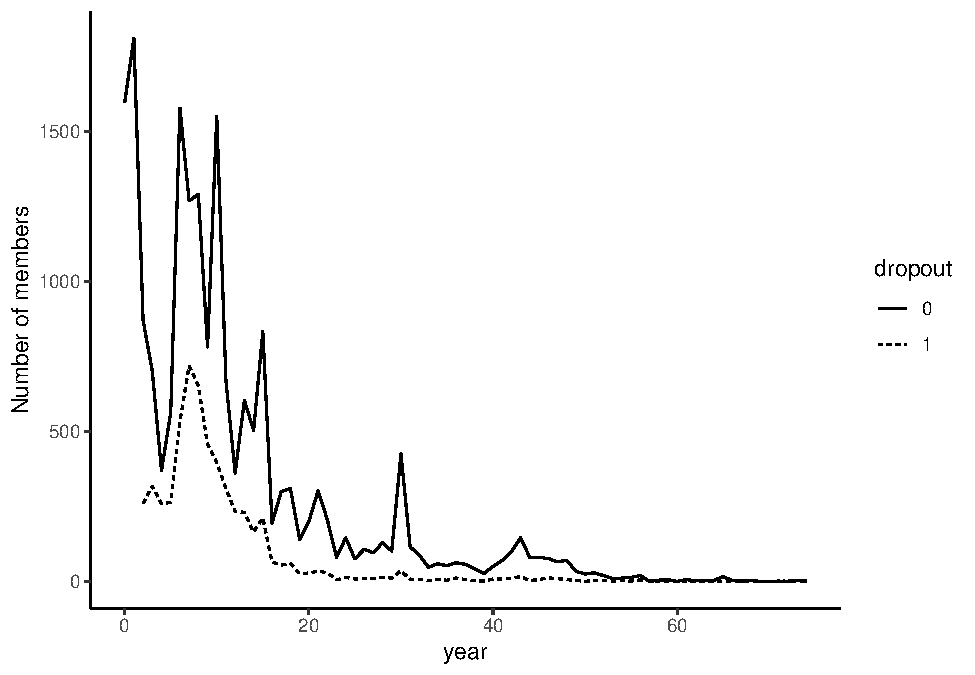
\includegraphics{articleCustomerDropoutMembership_files/figure-latex/membershipyear-1.pdf}
\caption{\label{fig:membershipyear}Number of members by year}
\end{figure}

\hypertarget{model-construction}{%
\subsection{Model construction}\label{model-construction}}

Address the model construction\ldots{} the categorical variables \(sex\),
\(marital\_status\) and \(quart\_stadium\_entries\) where converted to dummy
variables.

The random survival forest was developed using the package PySurvival
(\protect\hyperlink{ref-Fotso_others_2019}{Fotso et al. 2019}). The most relevant variables predicting the dropout are
analysed using the log-rank test. The metric variables are transformed to
categorical using the quartiles to provide a statistical comparison of groups.
The survival analysis was conducted using the package Lifelines
(\protect\hyperlink{ref-Davidson-Pilon_2021}{Davidson-Pilon 2021}).

PySurvival is an open source python package for Survival Analysis modeling - the
modeling concept used to analyze or predict when an event is likely to happen.
It is built upon the most commonly used machine learning packages such NumPy,
SciPy and PyTorch. PySurvival is compatible with Python 2.7-3.7

\hypertarget{survival-trees-based-model}{%
\subsubsection{Survival trees based model}\label{survival-trees-based-model}}

In this model\ldots{} The survival trees based model uses pysurvival random forest

Removed the variables with greater correlations \(total\_matches\) and
\(quart\_stadium\_entries\)

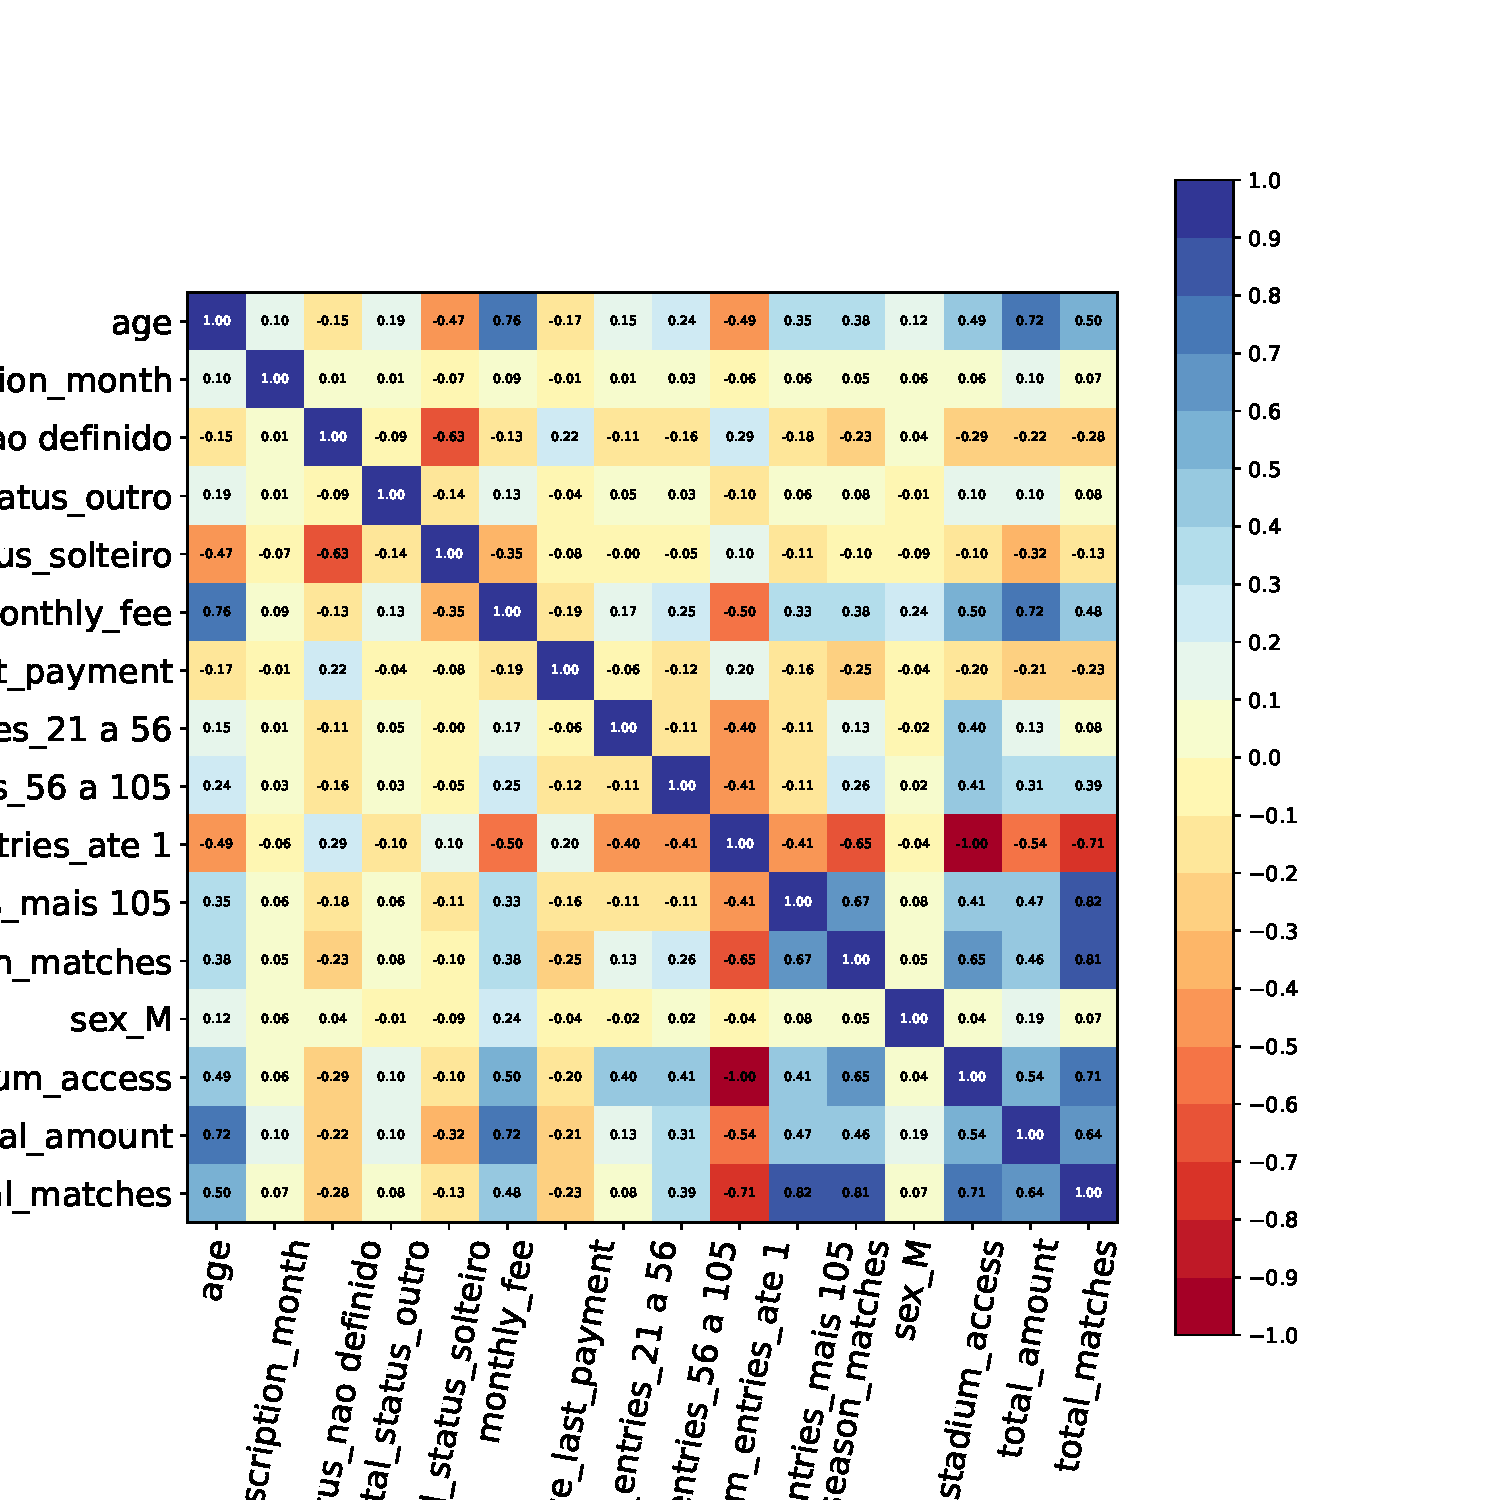
\includegraphics{articleCustomerDropoutMembership_files/figure-latex/removeVar-1.pdf}

\begin{verbatim}
##         age  ...  quart_stadium_entries_mais 105
## 0      83.0  ...                               0
## 1      88.0  ...                               0
## 2      73.0  ...                               0
## 3      97.0  ...                               0
## 4      97.0  ...                               0
## ...     ...  ...                             ...
## 25311   7.0  ...                               0
## 25312   8.0  ...                               0
## 25313   2.0  ...                               0
## 25314  14.0  ...                               0
## 25315  28.0  ...                               0
## 
## [25316 rows x 14 columns]
\end{verbatim}

\begin{verbatim}
## RandomSurvivalForestModel
\end{verbatim}

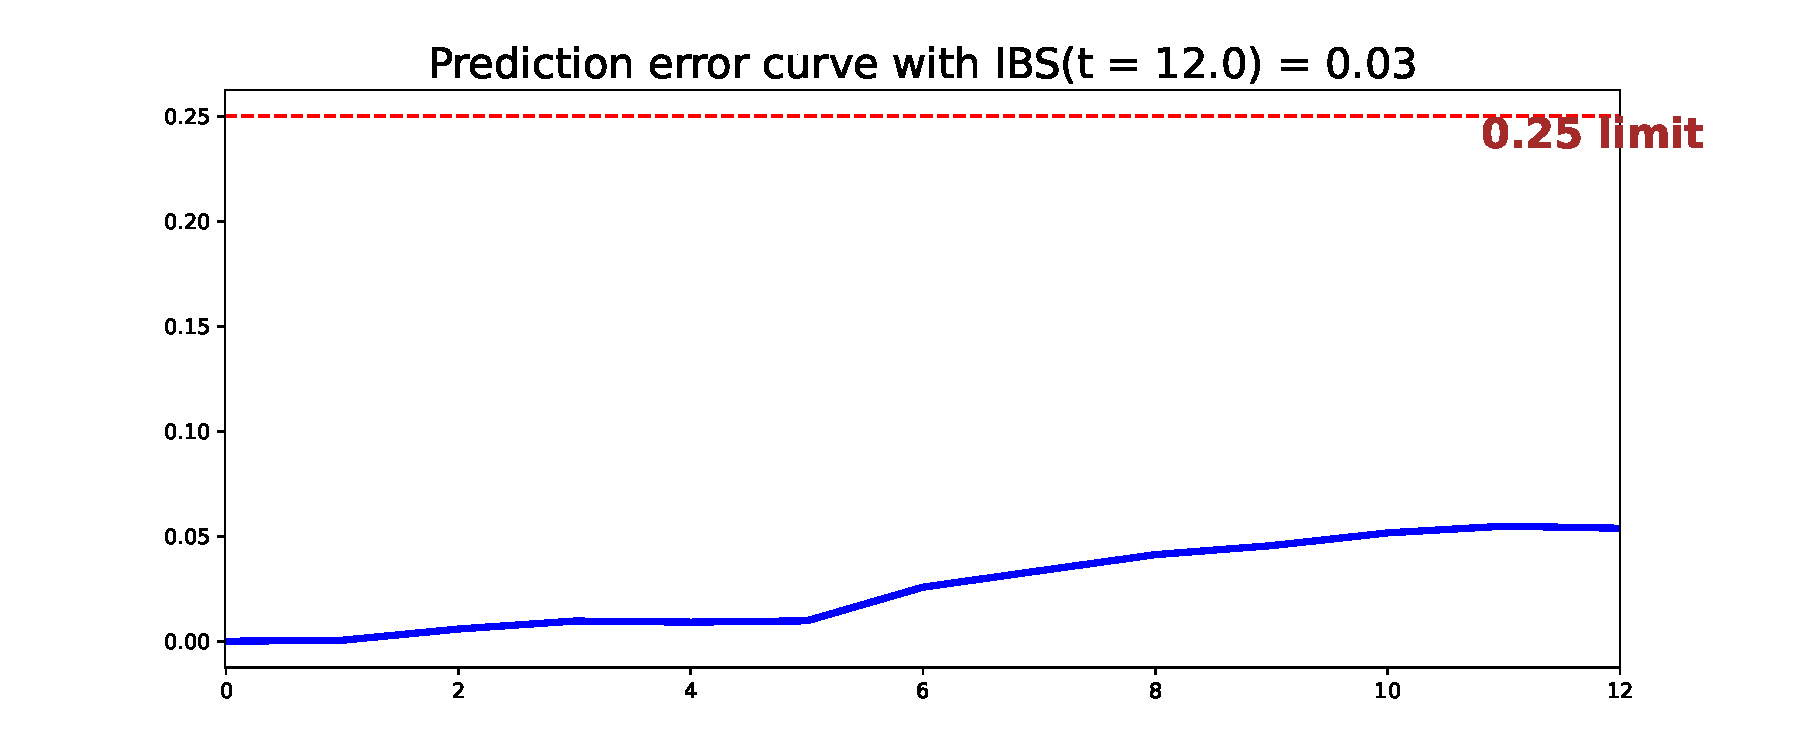
\includegraphics{articleCustomerDropoutMembership_files/figure-latex/createModel-3.pdf} 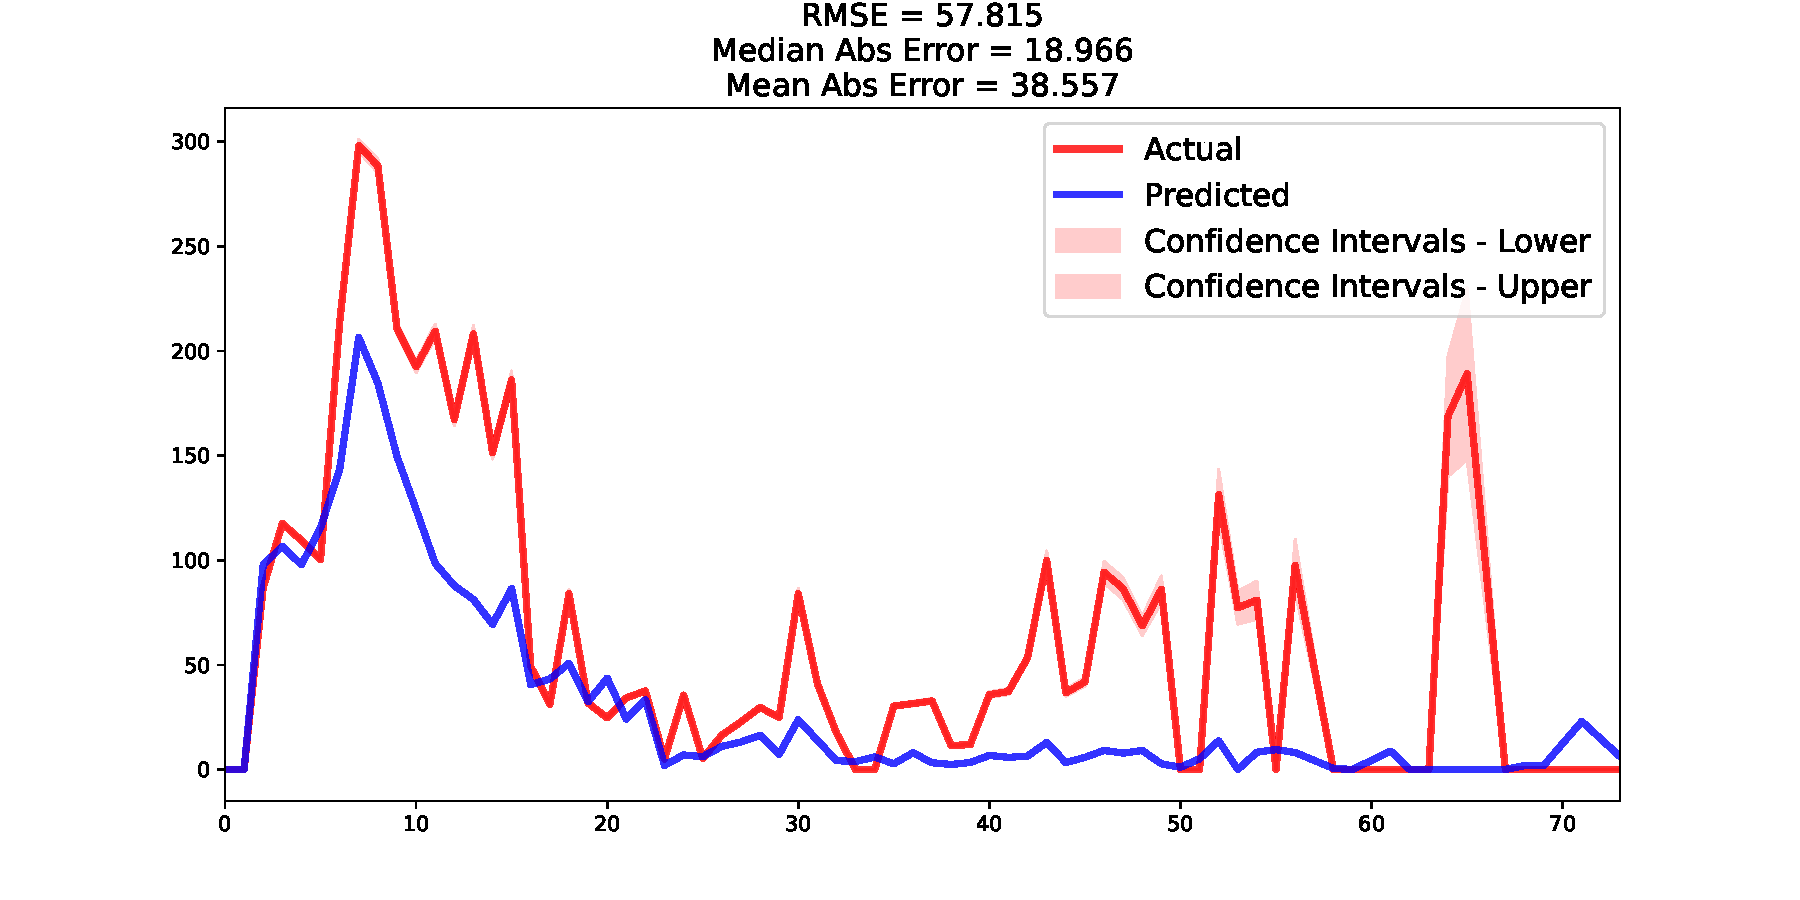
\includegraphics{articleCustomerDropoutMembership_files/figure-latex/createModel-4.pdf}

\begin{verbatim}
## {'root_mean_squared_error': 57.814697481046416, 'median_absolute_error': 18.96621852166039, 'mean_absolute_error': 38.55719494742953}
\end{verbatim}

Table \ref{tab:summarytable2} shows variables importance.

\begin{table}

\caption{\label{tab:summarytable2}Summary statistics of features used}
\centering
\begin{tabular}[t]{lrr}
\toprule
feature & importance & pct\_importance\\
\midrule
dropout & 6.0669405 & 0.2528415\\
months\_since\_last\_payment & 4.9581586 & 0.2066327\\
season\_matches & 2.3851555 & 0.0994020\\
total\_amount & 1.8950237 & 0.0789757\\
quart\_stadium\_entries\_21 a 56 & 1.4643279 & 0.0610263\\
\addlinespace
quart\_stadium\_entries\_56 a 105 & 1.3455565 & 0.0560765\\
stadium\_access & 1.2980882 & 0.0540982\\
inscription\_month & 1.2790920 & 0.0533065\\
marital\_status\_nao definido & 1.0339551 & 0.0430904\\
sex\_M & 0.8881565 & 0.0370142\\
\addlinespace
age & 0.7472122 & 0.0311403\\
monthly\_fee & 0.6333690 & 0.0263958\\
marital\_status\_solteiro & -0.2702218 & 0.0000000\\
marital\_status\_outro & -1.0259784 & 0.0000000\\
quart\_stadium\_entries\_mais 105 & -1.2762422 & 0.0000000\\
\addlinespace
years\_membership & -4.1258616 & 0.0000000\\
\bottomrule
\end{tabular}
\end{table}

\hypertarget{model-building}{%
\paragraph{Model building}\label{model-building}}

The model was built with with 70\% of the data for training and 30\% for testing.
The survival model parameters where:

The model accuracy is very high in the first years. The prediction is very
similar to the actual value. The absolute error mean of
39 customers.

\hypertarget{survival-trees-based-model-with-clusters}{%
\subsubsection{Survival trees based model with clusters}\label{survival-trees-based-model-with-clusters}}

Here we are will create clusters and developed the optimization within each
cluster\ldots{}

The calculation of he number of clusters used the package mclust (\protect\hyperlink{ref-scrucca2016}{Scrucca et al. 2016})
using the Bayesian Information Criterion (BIC). The model that gives the minimum
BIC score can be selected as the best model (\protect\hyperlink{ref-schwarz1978}{Schwarz 1978}) simplifying the
problem related to choosing the number of components and identifying the
structure of the covariance matrix, based on modelling with multivariate normal
distributions for each component that forms the data set (\protect\hyperlink{ref-akogul2016}{Akogul and Erisoglu 2016}).

In multivariate models are available the following approaches:

\begin{itemize}
\tightlist
\item
  ``EII''spherical, equal volume
\item
  ``EEE''ellipsoidal, equal volume, shape, and orientation
\item
  ``VII''spherical, unequal volume
\item
  ``VVV''ellipsoidal, varying volume, shape, and orientation, which is used as
  default for initialization of EM algorithm
\item
  VVI'': diagonal, varying volume and shape t
\end{itemize}

Estou a ter problemas com o cálculo dos clusters com o BIC\ldots{} estava a aqui a
confirmar os clusters, talvez seja melhor reduzir as variáveis\ldots{} testar a
abordagem aos clusters no artigo dos vinhos\ldots{}

\begin{Shaded}
\begin{Highlighting}[]
\FunctionTok{library}\NormalTok{(NbClust)}
\NormalTok{nb }\OtherTok{\textless{}{-}} \FunctionTok{NbClust}\NormalTok{(y, }\AttributeTok{diss=}\ConstantTok{NULL}\NormalTok{, }\AttributeTok{distance =} \StringTok{"euclidean"}\NormalTok{, }
              \AttributeTok{min.nc=}\DecValTok{2}\NormalTok{, }\AttributeTok{max.nc=}\DecValTok{5}\NormalTok{, }\AttributeTok{method =} \StringTok{"kmeans"}\NormalTok{, }
              \AttributeTok{index =} \StringTok{"all"}\NormalTok{, }\AttributeTok{alphaBeale =} \FloatTok{0.1}\NormalTok{)}
\FunctionTok{hist}\NormalTok{(nb}\SpecialCharTok{$}\NormalTok{Best.nc[}\DecValTok{1}\NormalTok{,], }\AttributeTok{breaks =} \FunctionTok{max}\NormalTok{(}\FunctionTok{na.omit}\NormalTok{(nb}\SpecialCharTok{$}\NormalTok{Best.nc[}\DecValTok{1}\NormalTok{,])))}
\end{Highlighting}
\end{Shaded}

\begin{verbatim}
## KMeans(n_clusters=1)
## KMeans(n_clusters=2)
## KMeans(n_clusters=3)
## KMeans(n_clusters=4)
## KMeans(n_clusters=5)
## KMeans(n_clusters=6)
## KMeans(n_clusters=7)
## KMeans()
## KMeans(n_clusters=9)
## KMeans(n_clusters=10)
## KMeans(n_clusters=11)
## KMeans(n_clusters=12)
## KMeans(n_clusters=13)
## KMeans(n_clusters=14)
## KMeans(n_clusters=15)
## KMeans(n_clusters=16)
## KMeans(n_clusters=17)
## KMeans(n_clusters=18)
## KMeans(n_clusters=19)
\end{verbatim}

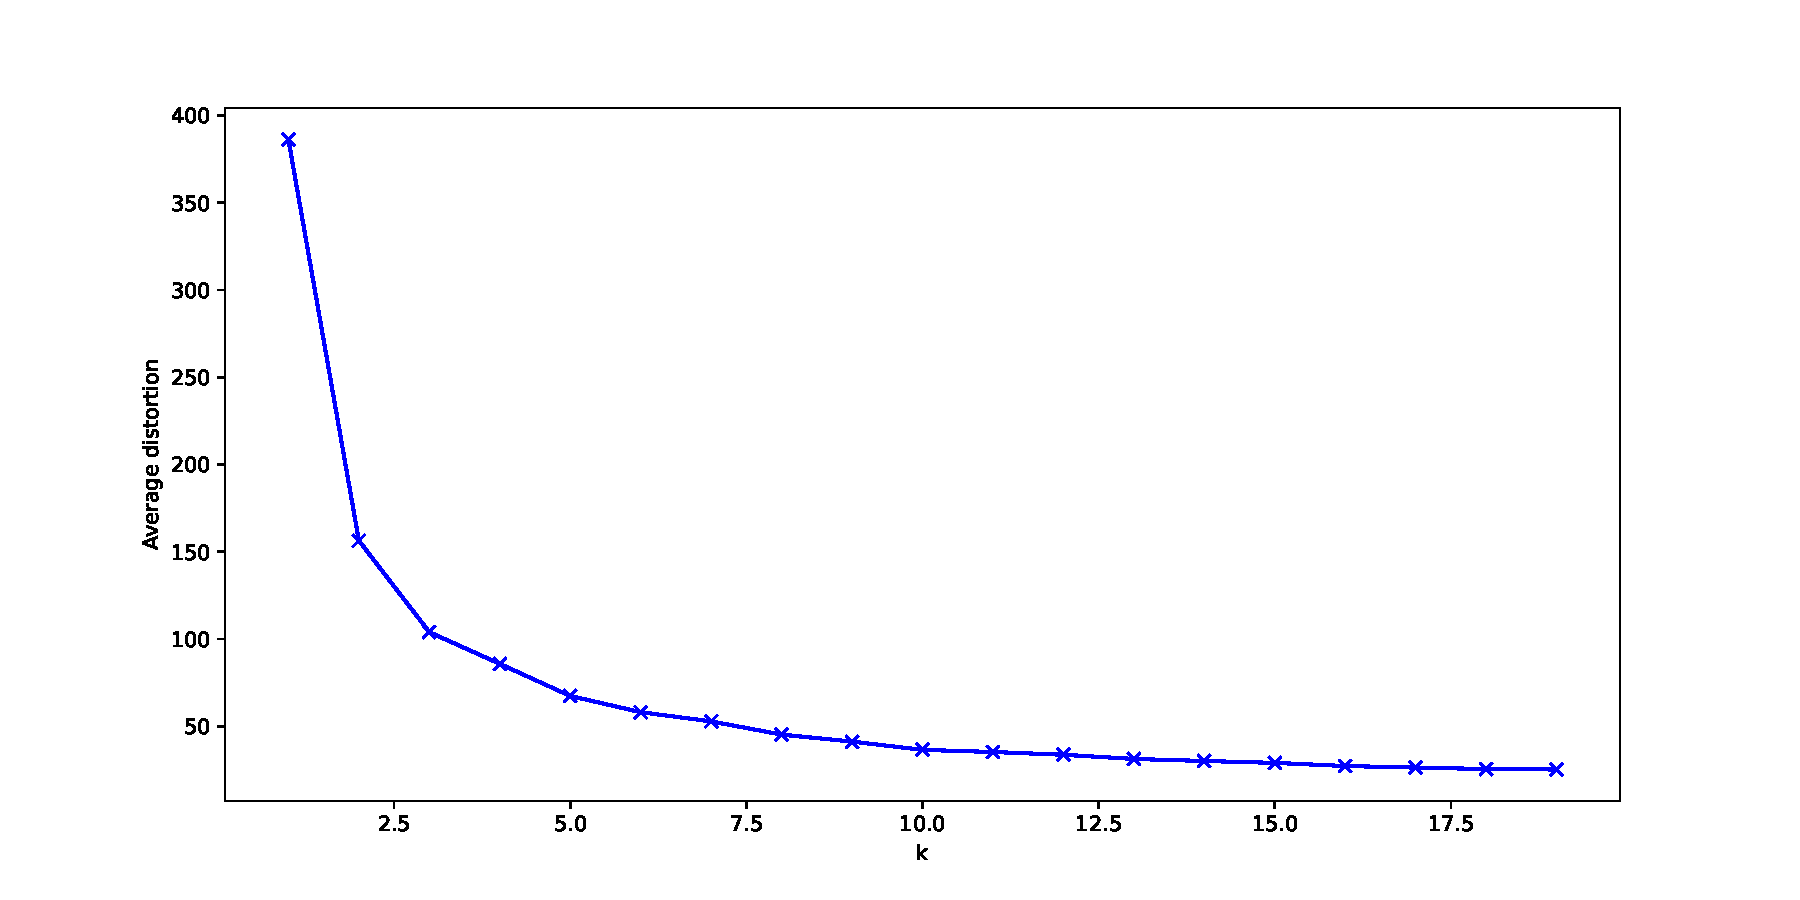
\includegraphics{articleCustomerDropoutMembership_files/figure-latex/elbowCalculation-1.pdf}

We are going to consider five clusters

\begin{verbatim}
## KMeans(n_clusters=5)
\end{verbatim}

\begin{verbatim}
## 1    17068
## 3     2818
## 2     2420
## 4     2080
## 0      930
## Name: cluster, dtype: int64
\end{verbatim}

TODO: Estava aqui\ldots{} fit the model for the five clusters\ldots{} compare the
performance with the model without clusters\ldots{} corrigir acima para selecionar só
as features.. Explorar t-SNE for better visualization\ldots{}

\begin{verbatim}
##        age  monthly_fee  total_amount  ...  cluster        X_pca     Y_pca
## 0     83.0         10.0        1906.0  ...        0  1591.733817  8.137428
## 1     88.0         10.0        1906.0  ...        0  1591.880351  8.064681
## 9     78.0         10.0        1901.0  ...        0  1586.569739  7.062815
## 11    71.0         10.0        1841.0  ...        0  1526.408306  7.138363
## 16    85.0         10.0        1846.0  ...        0  1531.809369  5.877420
## ...    ...          ...           ...  ...      ...          ...       ...
## 8395  38.0         10.0        1566.0  ...        0  1249.711939  0.672902
## 8448  76.0         10.0        1618.0  ...        0  1302.665956  9.866317
## 8527  46.0         10.0        1594.0  ...        0  1277.941830  1.814926
## 8820  35.0         10.0        1569.0  ...        0  1252.586502  1.828636
## 9618  50.0         10.0        1743.0  ...        0  1426.869737  8.847541
## 
## [930 rows x 17 columns]
## The cluster 0 as a size of 930
## RandomSurvivalForestModel
## Cluster 0 RMSE 2.7847832470895475
## Cluster 0 MAE 0.0
## Cluster 0 MAError 0.8993908970392324
##         age  monthly_fee  total_amount  ...  cluster        X_pca      Y_pca
## 2      73.0         10.0        1553.0  ...        4  1238.195691  36.216307
## 4      97.0         10.0        1466.0  ...        4  1151.973917  33.646937
## 8      88.0         10.0        1357.5  ...        4  1043.740627   1.126672
## 19     75.0         10.0        1330.0  ...        4  1015.805346  -0.159127
## 20     71.0         10.0        1202.0  ...        4   887.122902  43.078919
## ...     ...          ...           ...  ...      ...          ...        ...
## 13979  41.0         10.0        1055.0  ...        4   739.066765  -5.630017
## 14539  52.0         10.0        1160.0  ...        4   844.316227  -3.458902
## 14561  63.0         10.0        1054.0  ...        4   738.751223  -6.257051
## 14590  72.0         10.0        1054.0  ...        4   739.011833  -6.363162
## 14749  74.0         10.0        1176.0  ...        4   860.951124  -4.457038
## 
## [2080 rows x 17 columns]
## The cluster 4 as a size of 2080
## RandomSurvivalForestModel
## Cluster 4 RMSE 8.804563964516955
## Cluster 4 MAE 1.3491183838782987
## Cluster 4 MAError 3.724668251115418
##         age  monthly_fee  total_amount  ...  cluster       X_pca      Y_pca
## 3      97.0          5.0         790.0  ...        2  476.781177  -2.878081
## 5      91.0          5.0         805.0  ...        2  491.654217  -6.574167
## 6      88.0          5.0         615.0  ...        2  301.161262  27.733634
## 12     89.0          5.0         725.0  ...        2  411.433840   5.239050
## 13     92.0          5.0         825.0  ...        2  511.634603  -7.411714
## ...     ...          ...           ...  ...      ...         ...        ...
## 18969  36.0         10.0         592.5  ...        2  276.710745 -13.295363
## 18995  29.0         10.0         605.0  ...        2  288.882087  -5.939539
## 19065  65.0         10.0         618.0  ...        2  303.058407 -13.402052
## 19138  52.0         10.0         594.0  ...        2  278.671061 -13.549406
## 19416  34.0         10.0         646.0  ...        2  330.084474 -11.496563
## 
## [2423 rows x 17 columns]
## The cluster 2 as a size of 2423
## RandomSurvivalForestModel
## Cluster 2 RMSE 15.081809157987264
## Cluster 2 MAE 1.9948683372618339
## Cluster 2 MAError 6.859660105558099
##         age  monthly_fee  total_amount  ...  cluster       X_pca      Y_pca
## 7      95.0          5.0         340.0  ...        3   26.565346  22.744681
## 10     95.0          5.0         560.0  ...        3  246.434943  22.798580
## 18     86.0          5.0         580.0  ...        3  266.594554 -10.865739
## 31     89.0          5.0         580.0  ...        3  266.622206 -10.015085
## 43     83.0          5.0         530.0  ...        3  216.549443 -11.924744
## ...     ...          ...           ...  ...      ...         ...        ...
## 22880  55.0         10.0         215.0  ...        3 -100.027020 -17.220179
## 22889  23.0         10.0         215.0  ...        3 -101.020945 -13.716401
## 22979  39.0         10.0         215.0  ...        3 -100.531227 -16.812108
## 23367  31.0         10.0         210.0  ...        3 -105.731921 -17.904987
## 23594  60.0         10.0         225.0  ...        3  -89.927650 -17.890924
## 
## [2816 rows x 17 columns]
## The cluster 3 as a size of 2816
## RandomSurvivalForestModel
## Cluster 3 RMSE 9.353790515157675
## Cluster 3 MAE 2.5063338932739687
## Cluster 3 MAError 6.426789920472172
##         age  monthly_fee  total_amount  ...  cluster       X_pca       Y_pca
## 1315   54.0         10.0           0.0  ...        1 -314.381393  -22.760221
## 1607   58.0         10.0           5.0  ...        1 -311.253206  111.949308
## 1722   50.0         10.0           0.0  ...        1 -314.586559  -22.906591
## 1723   43.0         10.0           0.0  ...        1 -314.792159  -22.808044
## 1724   47.0         10.0           0.0  ...        1 -314.674673  -22.864357
## ...     ...          ...           ...  ...      ...         ...         ...
## 25311   7.0          1.0          17.0  ...        1 -299.395699  -21.087144
## 25312   8.0          1.0          12.0  ...        1 -304.362982  -21.171984
## 25313   2.0          1.0          17.0  ...        1 -299.542555  -21.016754
## 25314  14.0          1.0          17.0  ...        1 -299.190099  -21.185691
## 25315  28.0         10.0           0.0  ...        1 -315.721037  -21.659490
## 
## [17067 rows x 17 columns]
## The cluster 1 as a size of 17067
## RandomSurvivalForestModel
## Cluster 1 RMSE 78.14078277695158
## Cluster 1 MAE 28.53685333800375
## Cluster 1 MAError 56.988744683732826
\end{verbatim}

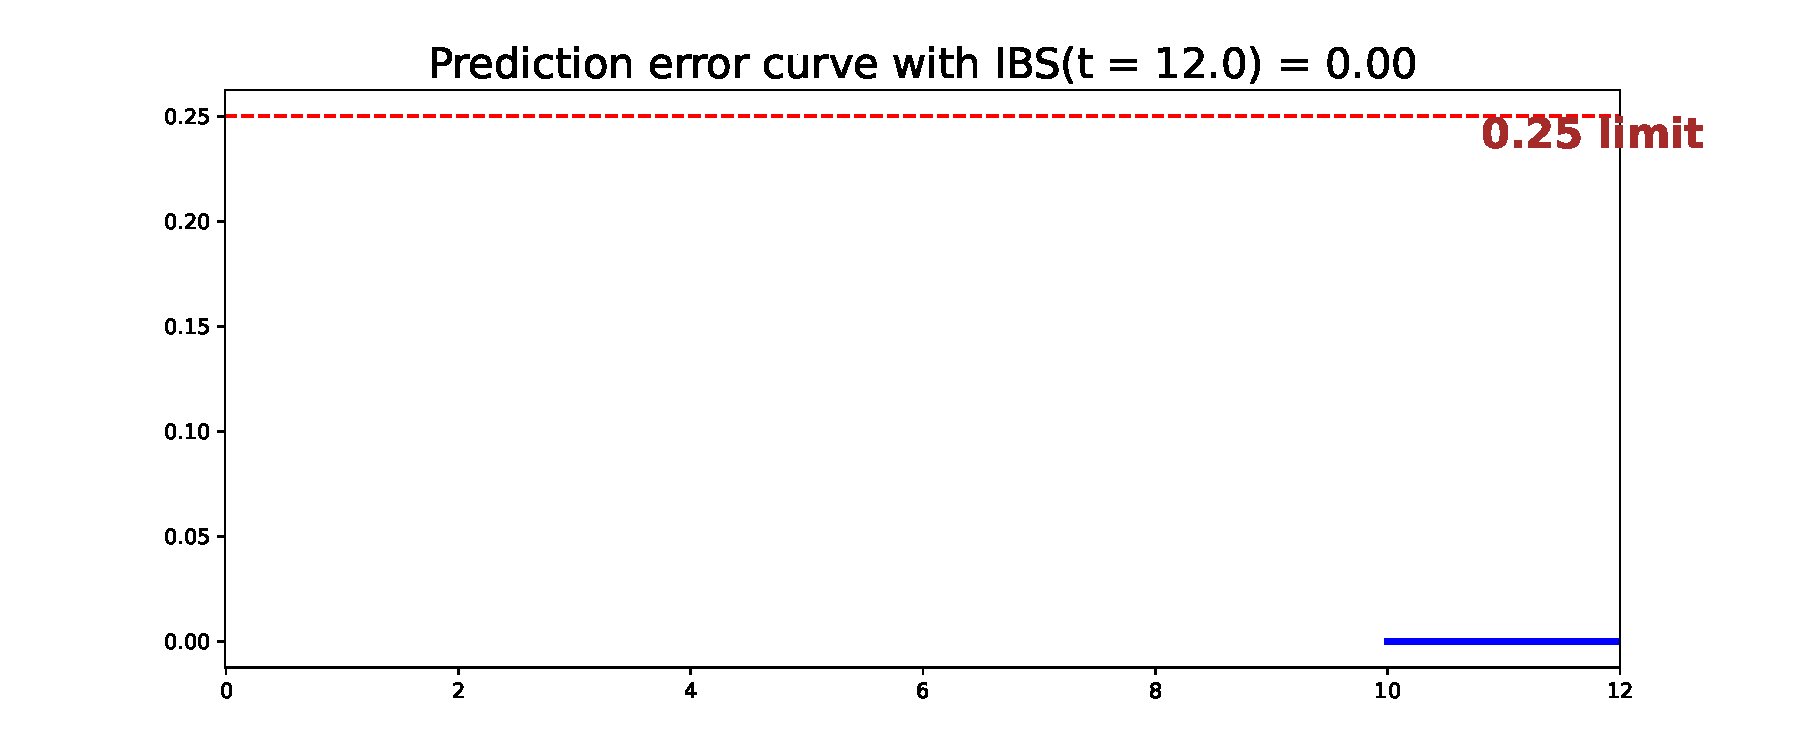
\includegraphics{articleCustomerDropoutMembership_files/figure-latex/createModelClusters-3.pdf} 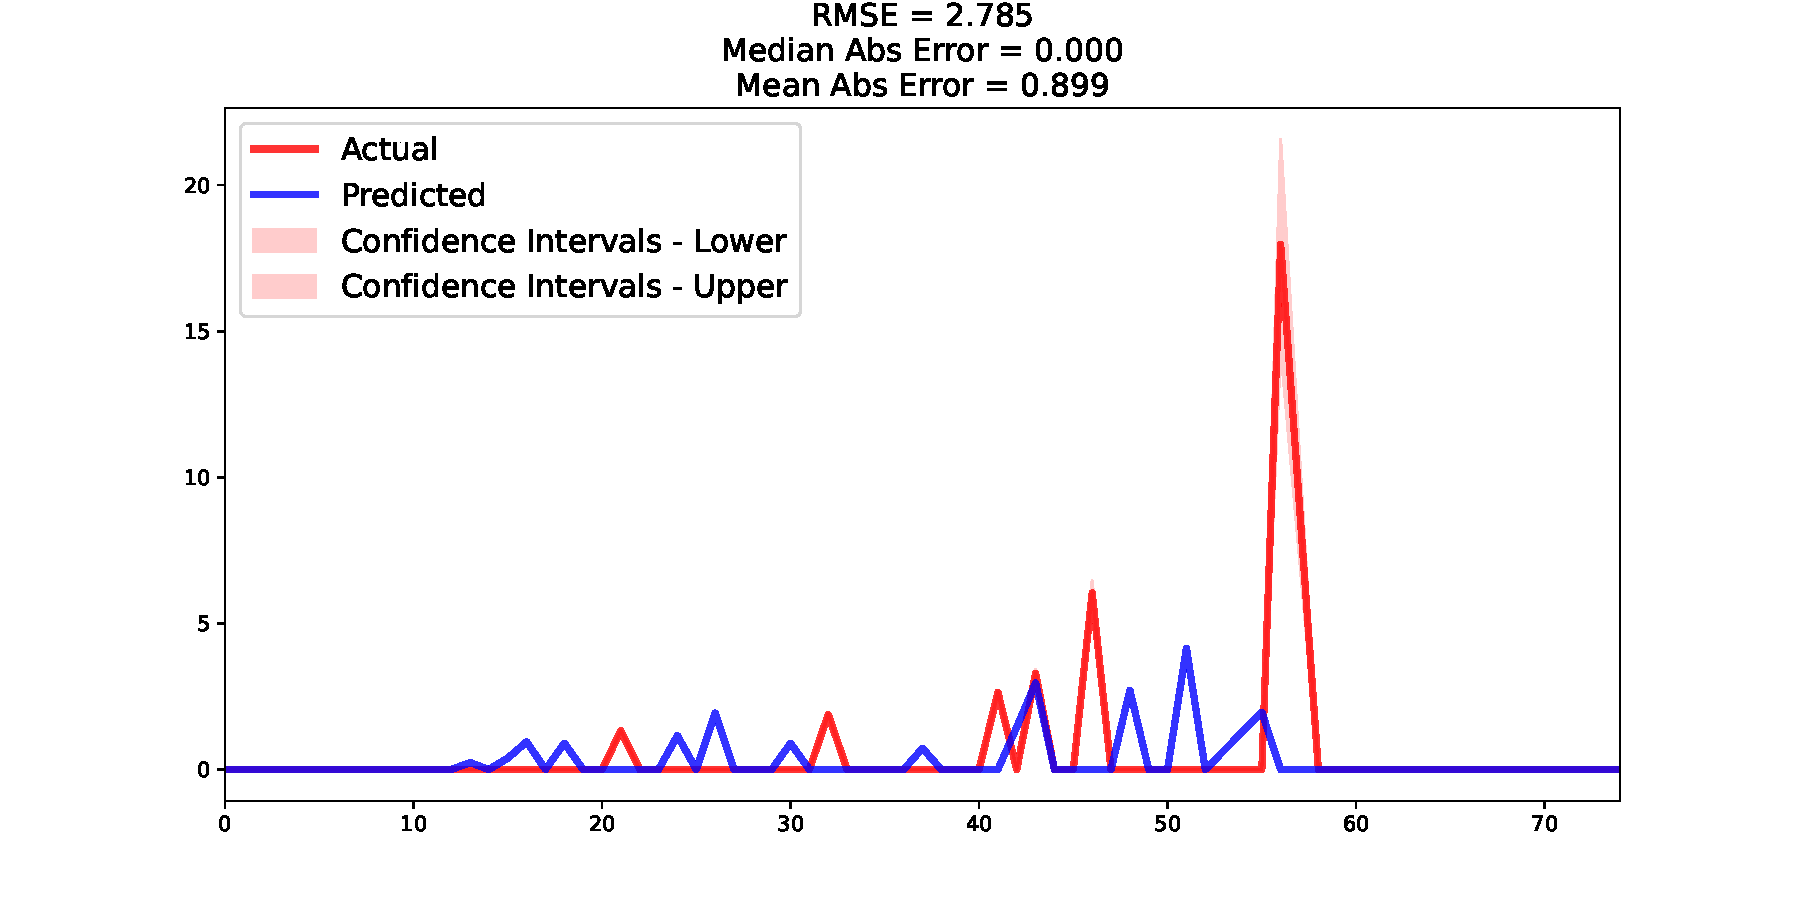
\includegraphics{articleCustomerDropoutMembership_files/figure-latex/createModelClusters-4.pdf} 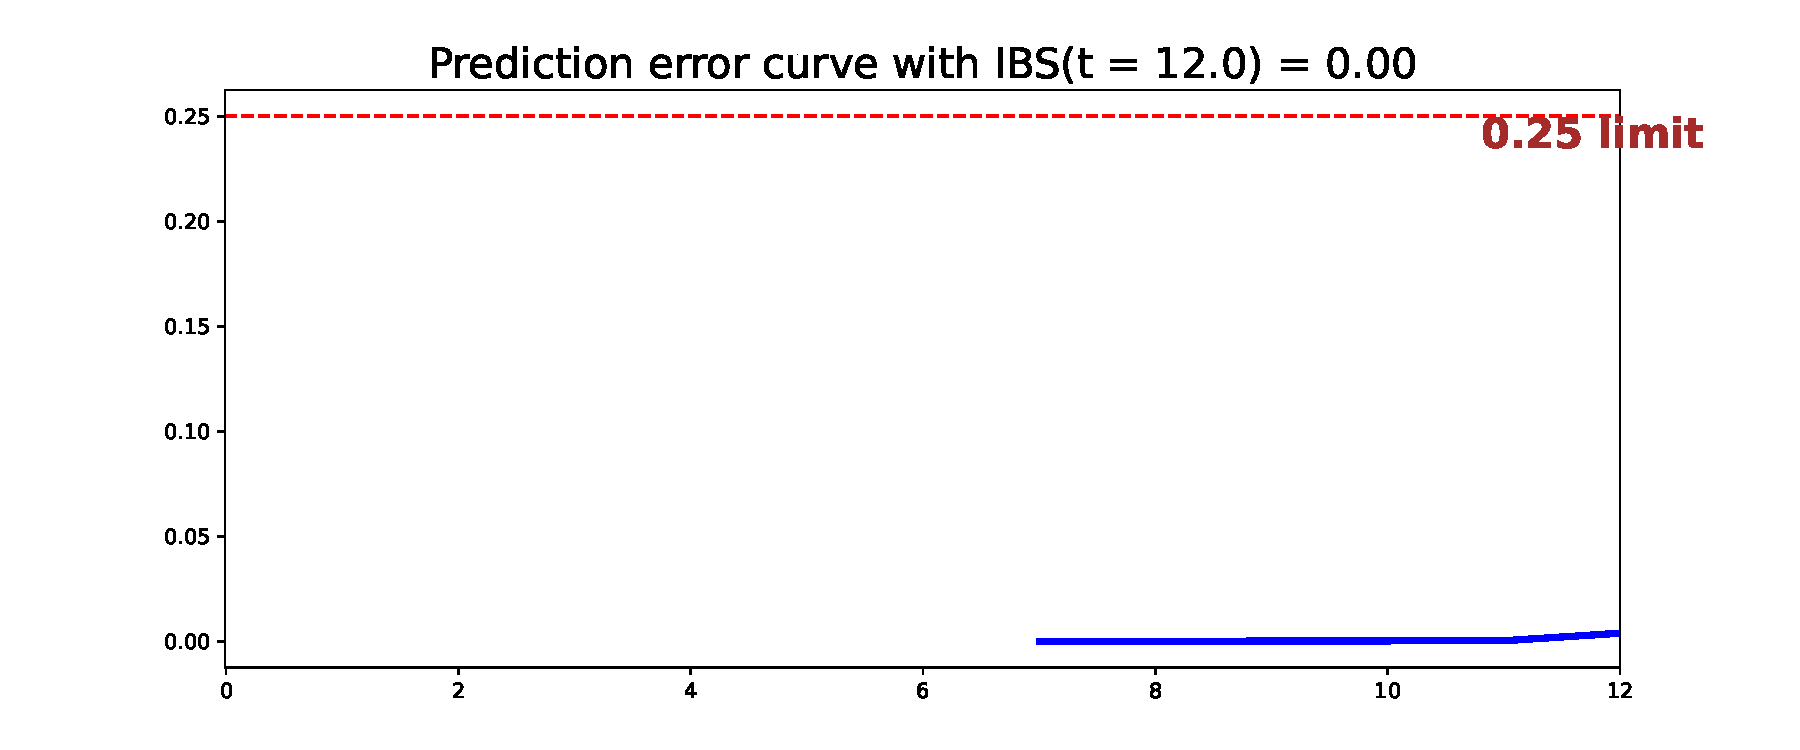
\includegraphics{articleCustomerDropoutMembership_files/figure-latex/createModelClusters-5.pdf} 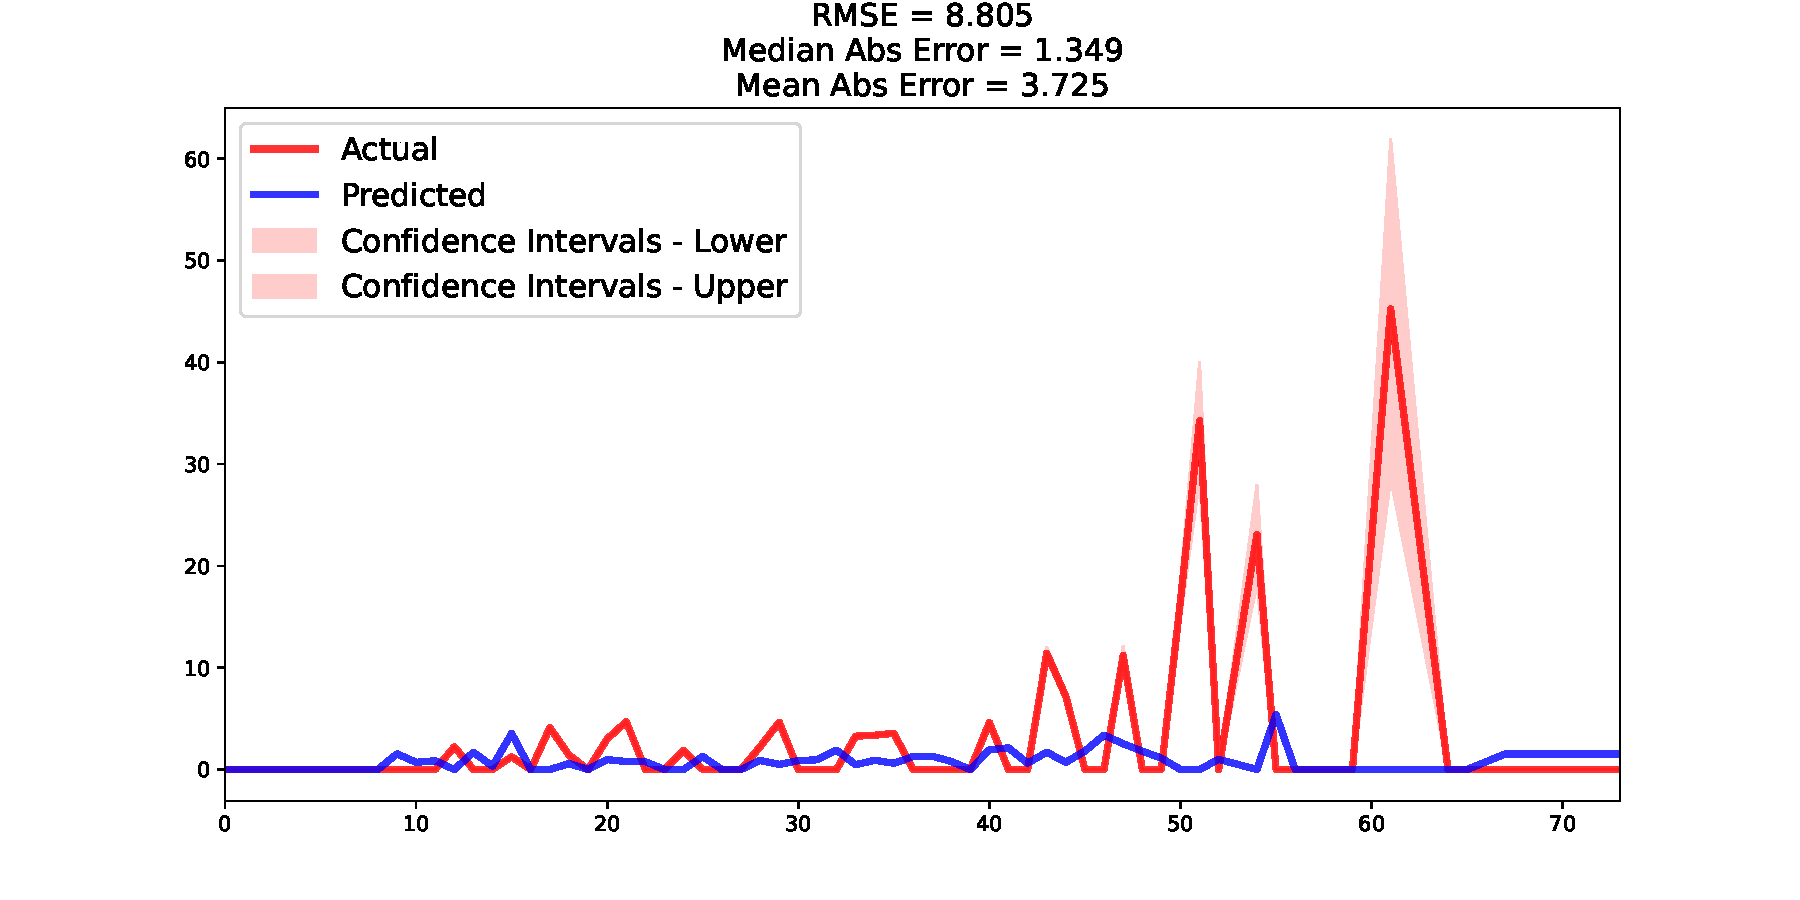
\includegraphics{articleCustomerDropoutMembership_files/figure-latex/createModelClusters-6.pdf} 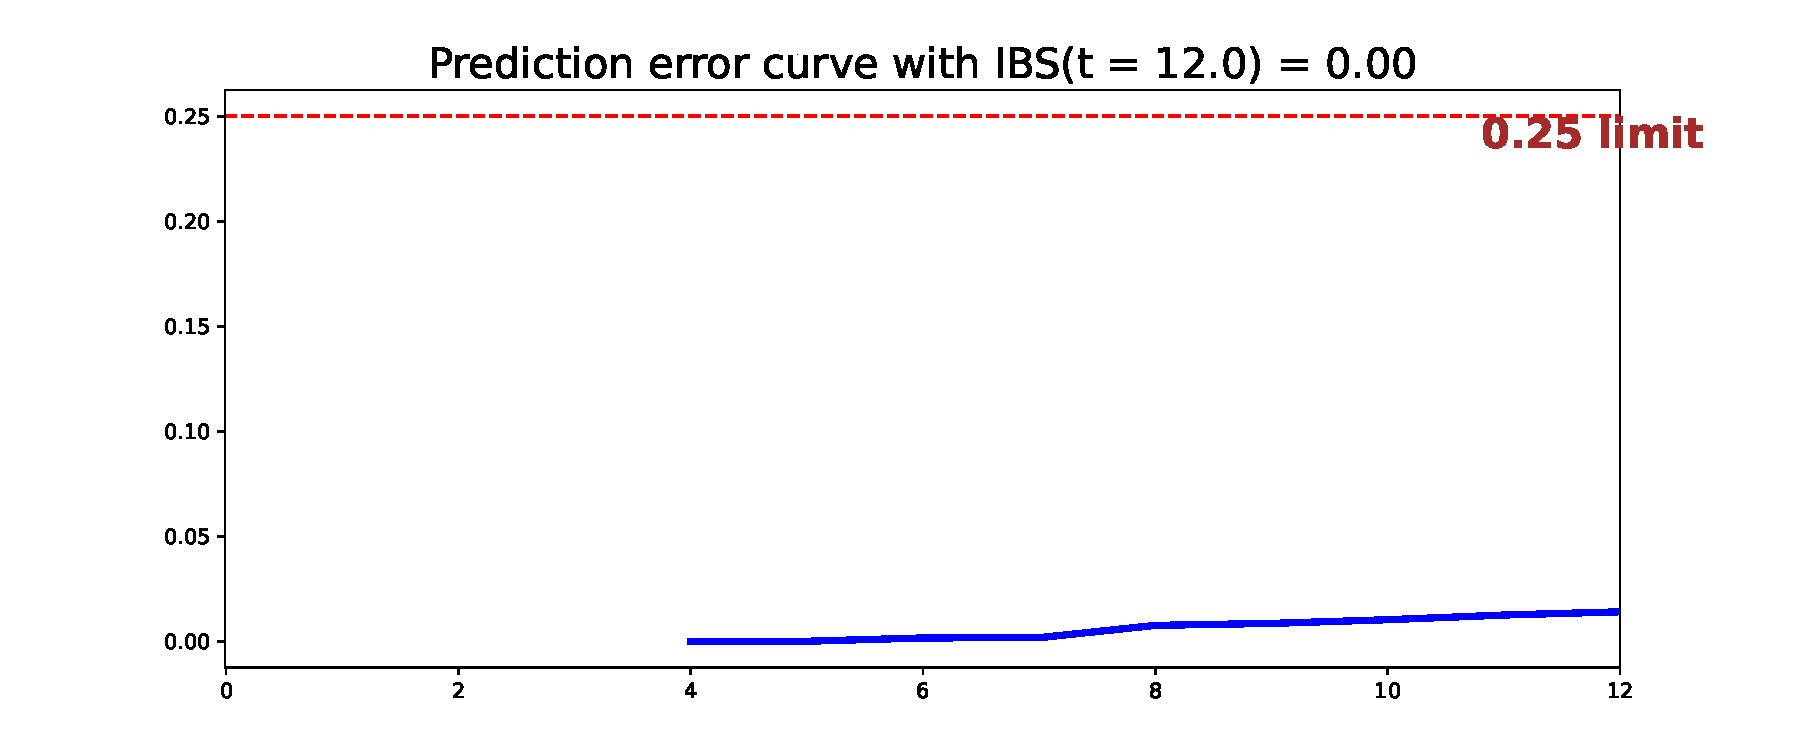
\includegraphics{articleCustomerDropoutMembership_files/figure-latex/createModelClusters-7.pdf} 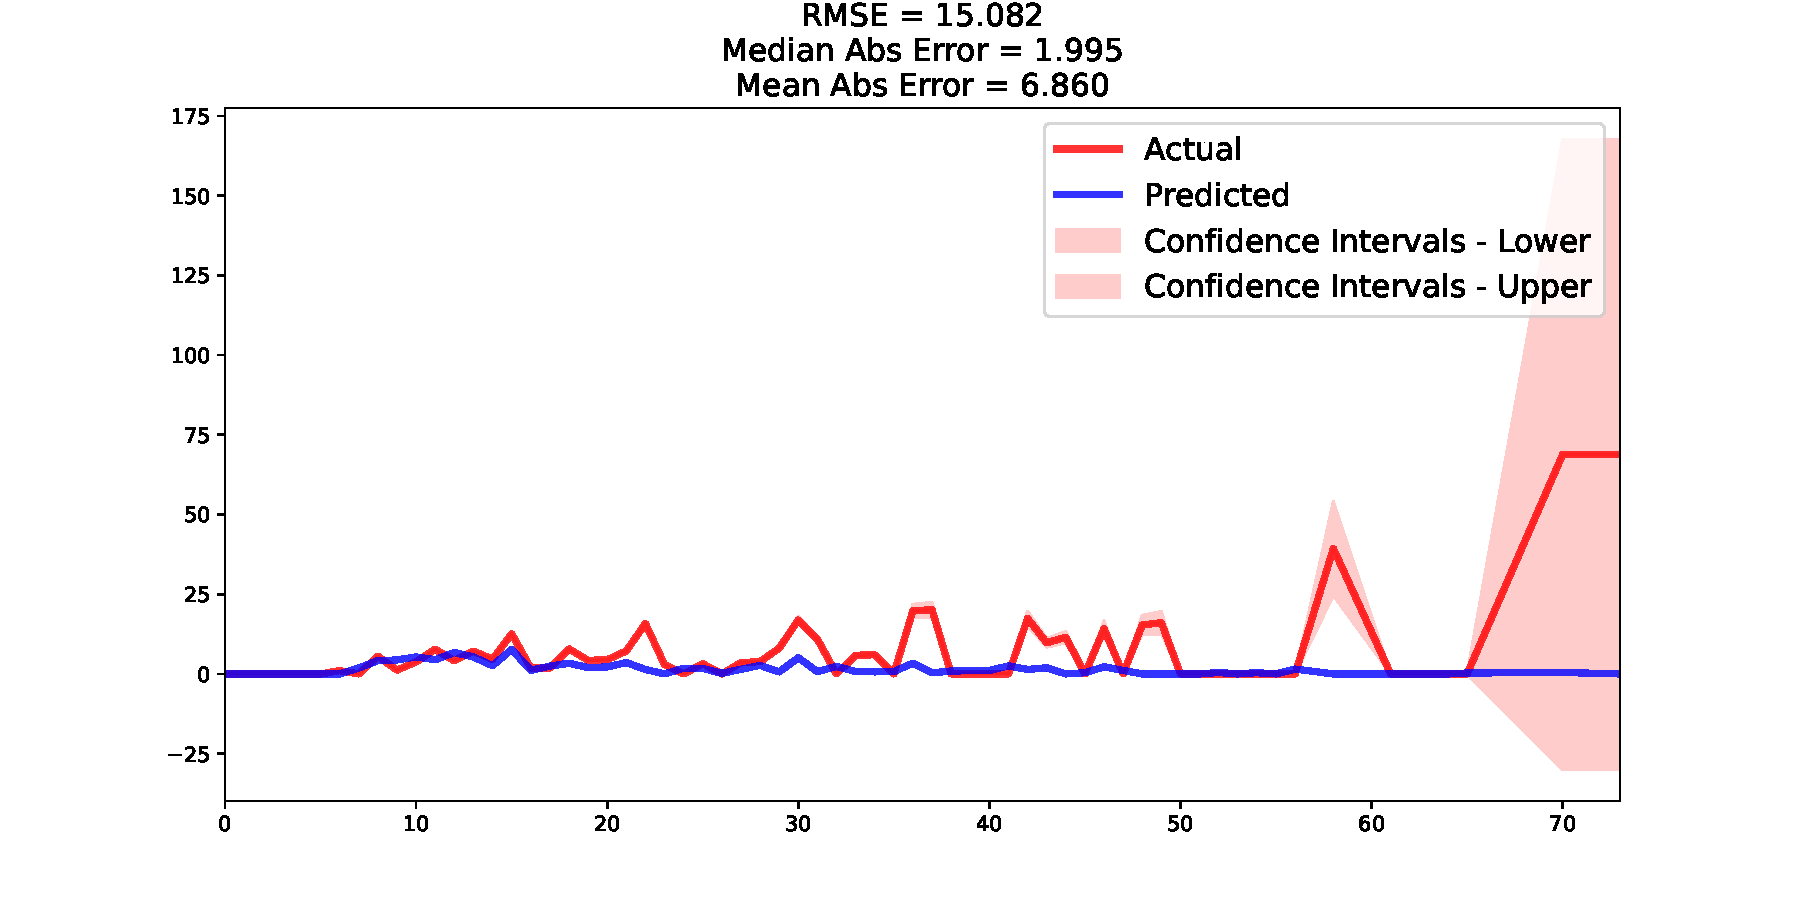
\includegraphics{articleCustomerDropoutMembership_files/figure-latex/createModelClusters-8.pdf} 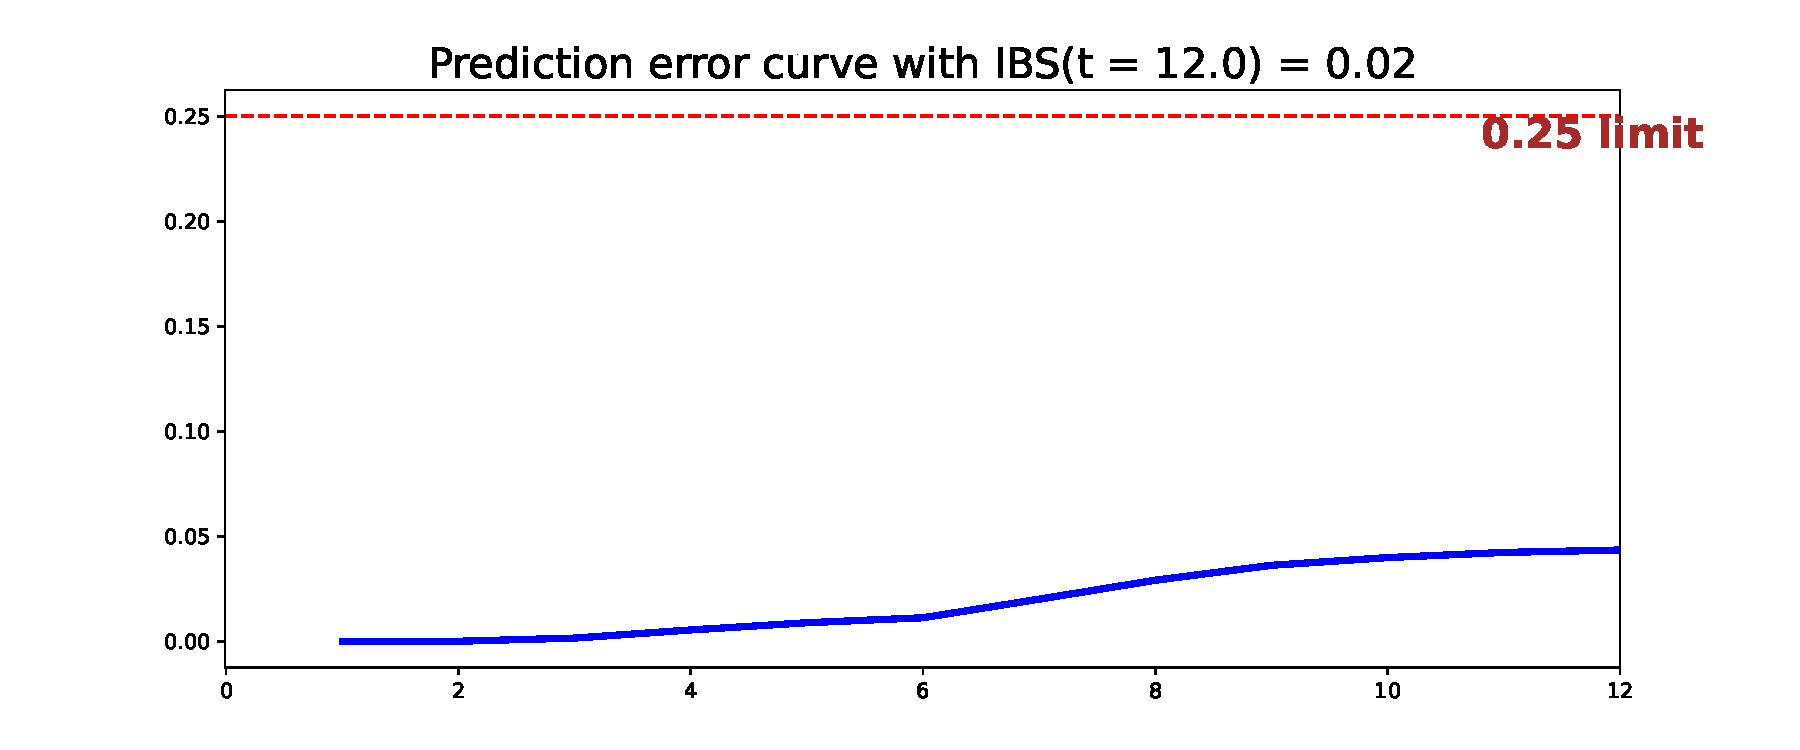
\includegraphics{articleCustomerDropoutMembership_files/figure-latex/createModelClusters-9.pdf} 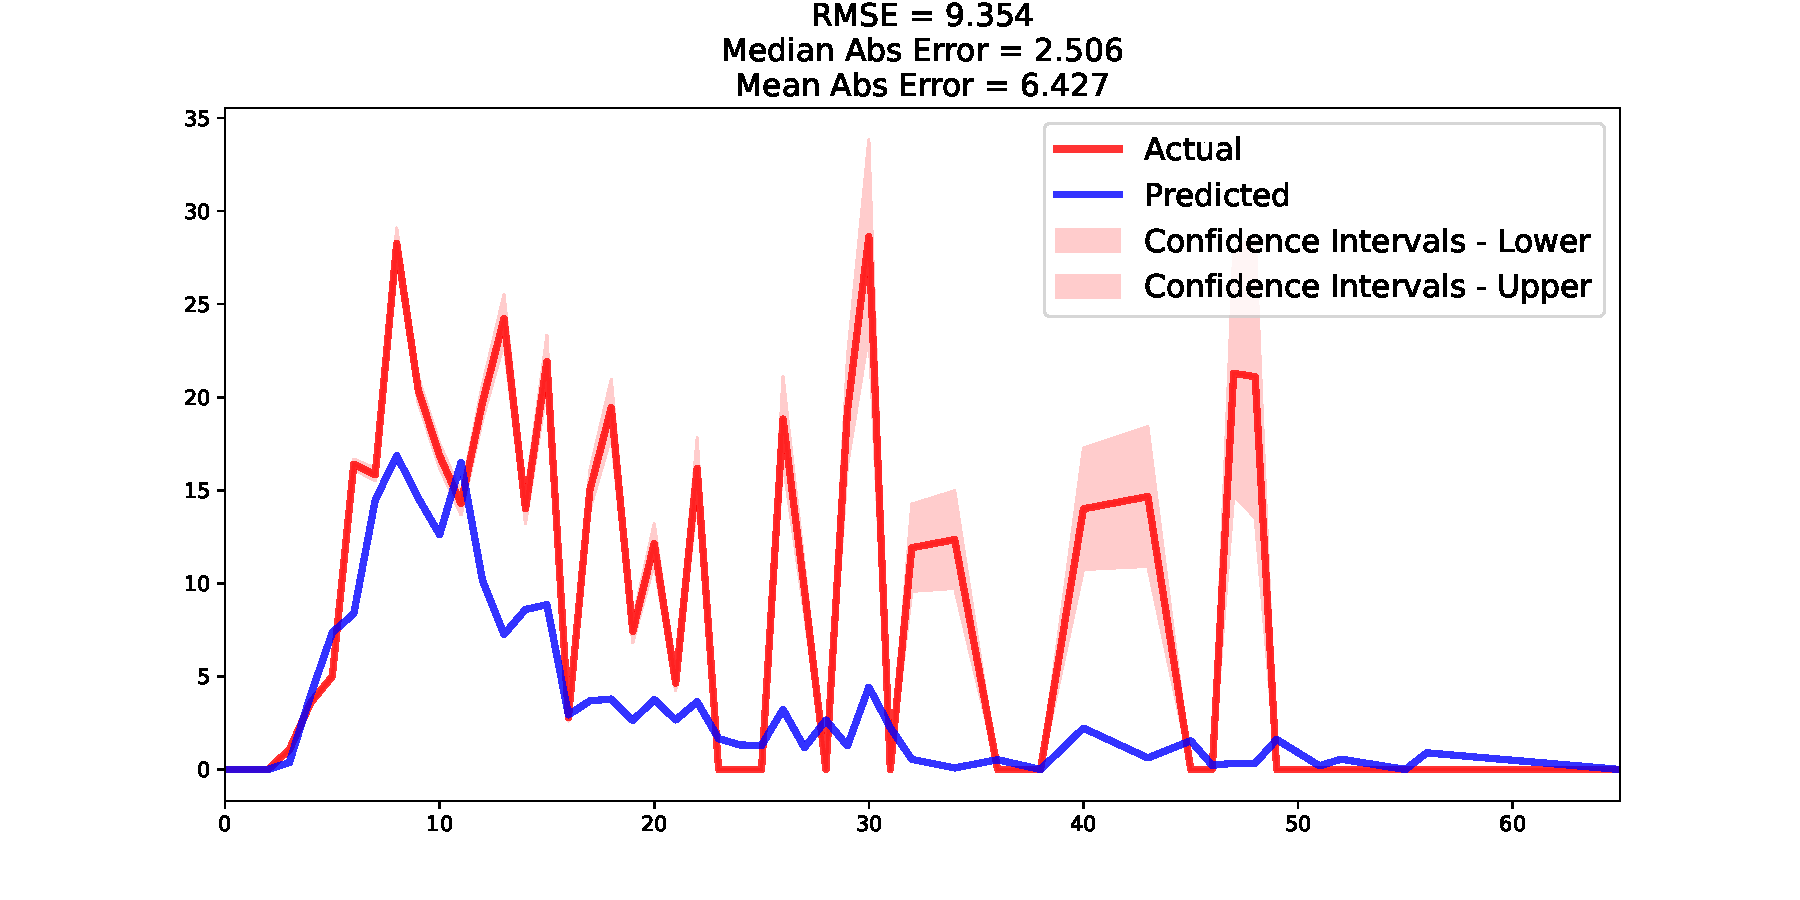
\includegraphics{articleCustomerDropoutMembership_files/figure-latex/createModelClusters-10.pdf} 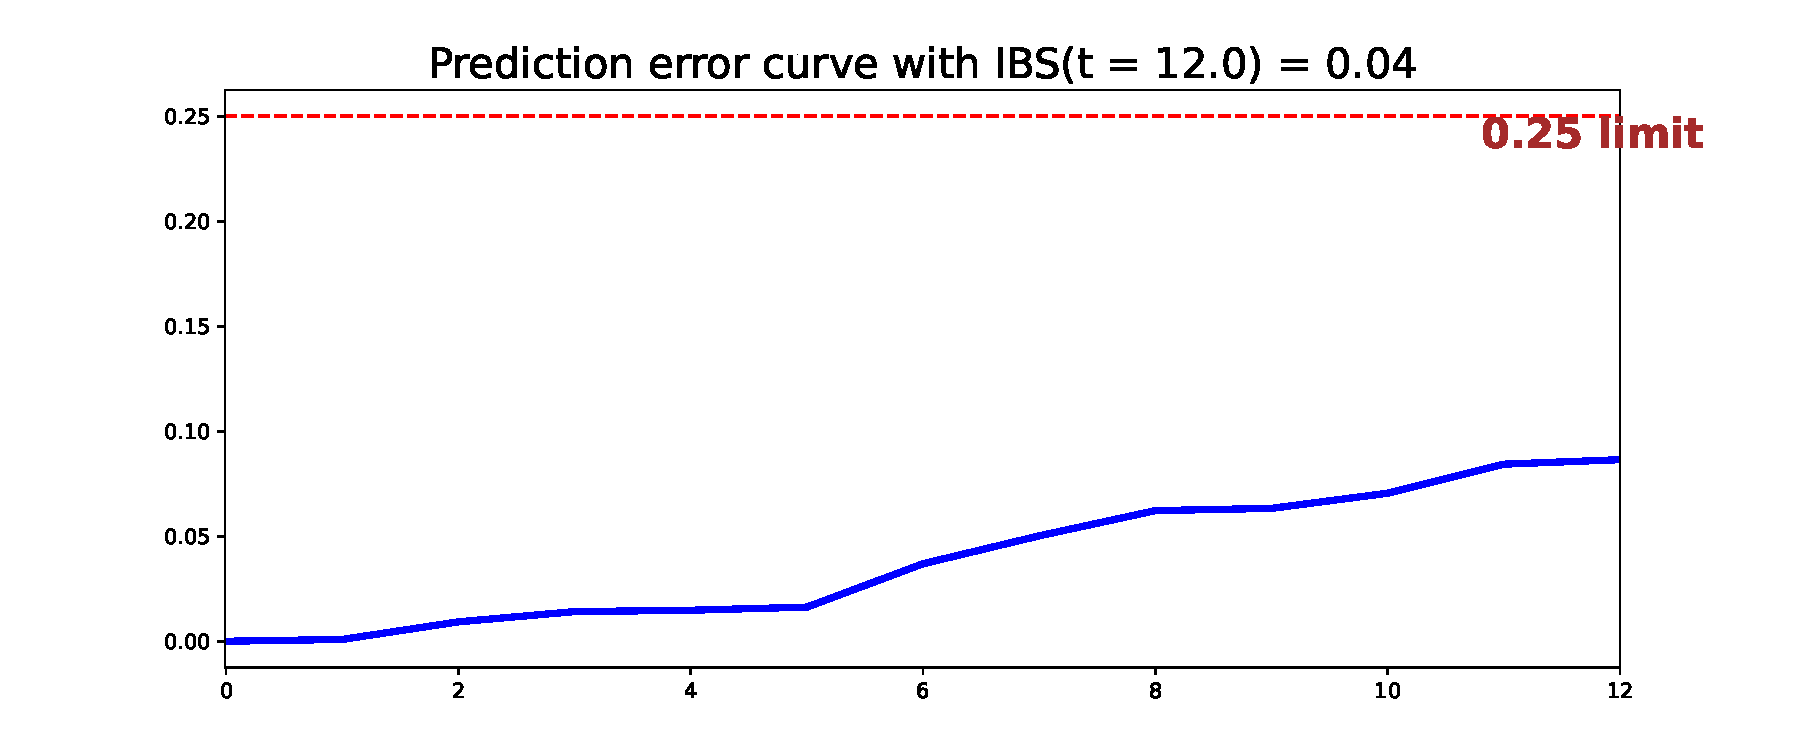
\includegraphics{articleCustomerDropoutMembership_files/figure-latex/createModelClusters-11.pdf} 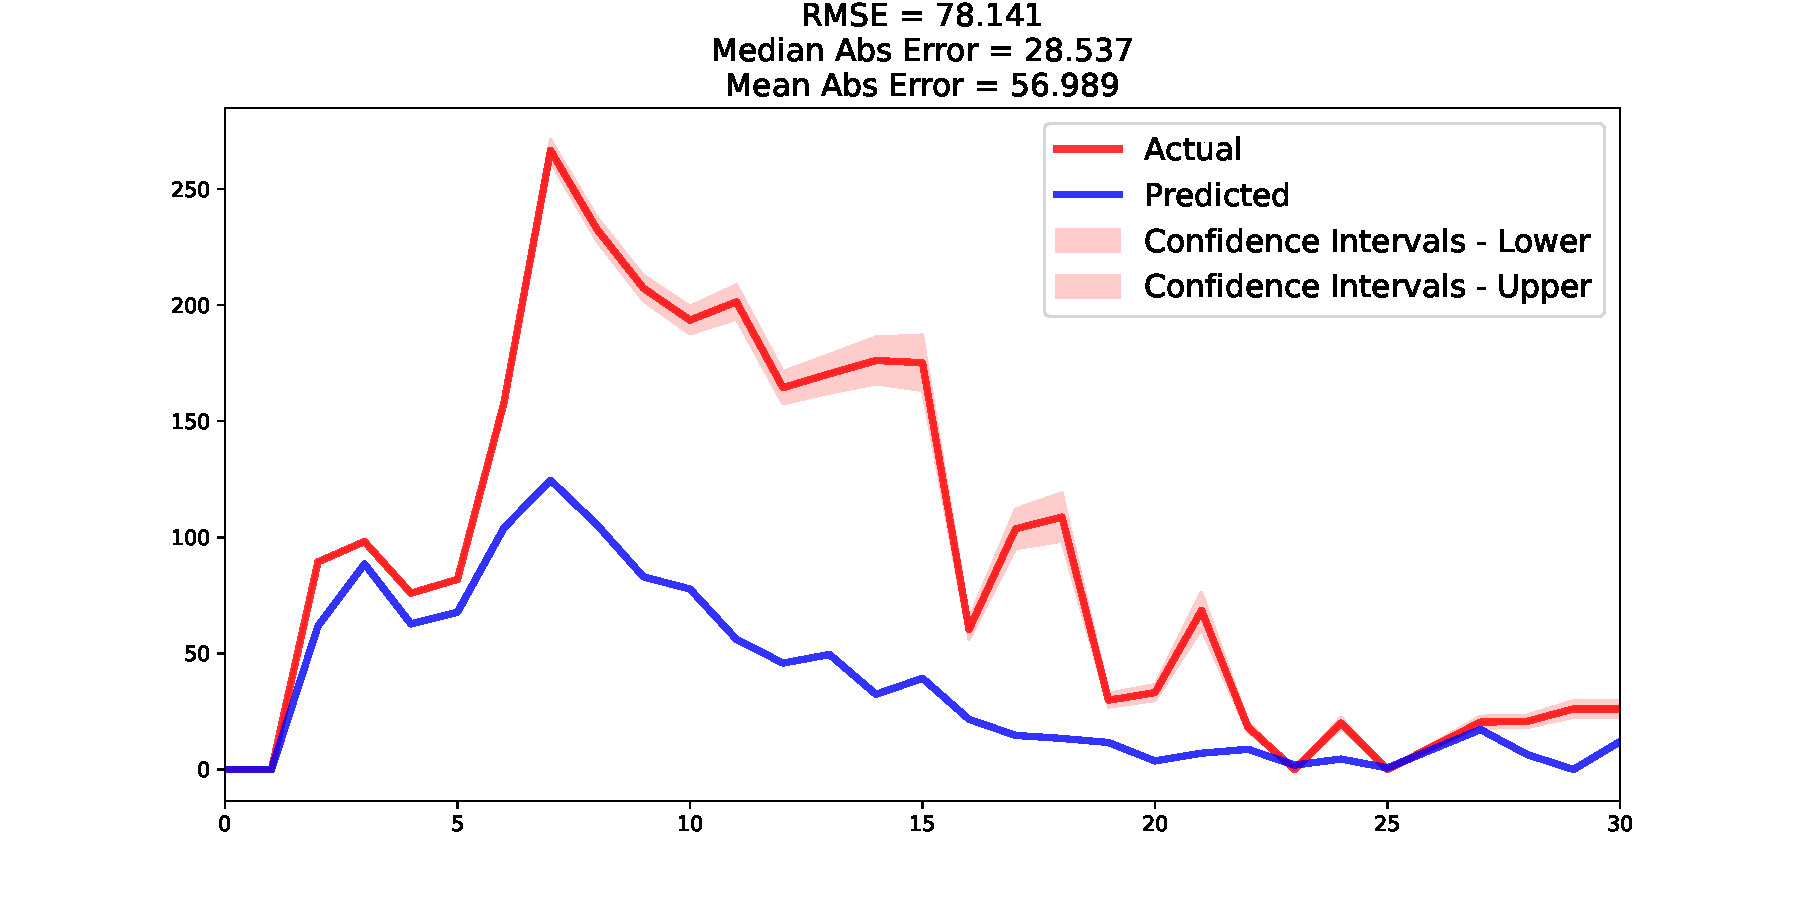
\includegraphics{articleCustomerDropoutMembership_files/figure-latex/createModelClusters-12.pdf}

\hypertarget{open-questions---to-remove}{%
\section{Open questions - to remove}\label{open-questions---to-remove}}

\begin{itemize}
    \item RQ1: What is the current state of the research being developed?
    \item RQ2: What algorithms have been used to predict dropout?
    \item RQ3: What are the features used to predict dropout?
    \item RQ4: When does dropout occur?
    \item RQ5: How is the accuracy of the machine learning algorithms in predicting dropout measured?
\end{itemize}

From RQ1, it was possible to identify some business areas that are
under-researched, such as the energy sector, education, logistics and
hospitality. Compared to other business areas such telecom or the financial
sector, research on the energy sector or water supply is lacking, considering
the contractual settings that are assumed to provide such types of services.
Considering the business model of many software companies as software as a
services (SaS), the number of research works is also surprisingly low.

RQ2 also provided an overall perspective related to the algorithms being used to
predict customer dropout. The first could be the importance and wider adoption
of decision trees and random forests (\protect\hyperlink{ref-antipov_applying_2010}{Antipov and Pokryshevskaya 2010}; \protect\hyperlink{ref-benoit_improving_2012}{Benoit and Van den Poel 2012}; \protect\hyperlink{ref-burez_crm_2007}{Burez and Van den Poel 2007}), and logistic regression
(\protect\hyperlink{ref-coussement_improved_2010}{Coussement, Benoit, and Van den Poel 2010}), which could be due to its higher interpretability
and flexibility (\protect\hyperlink{ref-keramati_improved_2014}{Keramati et al. 2014}). Interpretability is an important
aspect for the marketing department in the extraction of valuable information
from the model to develop effective retention strategies (\protect\hyperlink{ref-verbeke_new_2012}{Verbeke et al. 2012}).
The problem arises in the balancing between interpretability and the higher
performance of the algorithms inspired by nature (such as neural networks). From
a business perspective, dropout prediction should also be considered as a
business objective, which requires more than predicting if the customer will
churn or not (\protect\hyperlink{ref-devriendt_why_2019}{Devriendt et al. 2019}), where higher interpretability provides
better support in the development of retention strategies. The developed SLR
also raises the possibility of integrating different algorithms using ensemble
methods or integrating several models using a hybrid approach. None of the
studies integrated the survival approach to predict customer dropout, for
example, using a hybrid approach.

It is considered positive if actions are developed to retain customers, but the
problems should also be considered, such as the following: (1) customers who
have greater risk of dropout should be targeted to provide a base for a better
ROI in the retention strategies (\protect\hyperlink{ref-coussement_churn_2008}{Coussement and Van den Poel 2008}; \protect\hyperlink{ref-xie_customer_2009}{Xie et al. 2009}) and
(2) the retention strategies should be developed focused on customers with
higher satisfaction, or its inclusion could be a reminder of the contractual
agreement nearing an end and could lead to churn (\protect\hyperlink{ref-devriendt_why_2019}{Devriendt et al. 2019}).

From RQ3, several types of features being used were able to be identified, such
as demographic, behavioral, and economic indicators, pictorial data, network
relationships or high cardinality features. The problem that arises is that some
studies used data and features that were not described, and this creates a major
issue, How can reproducibility be developed in a study without the availability
of the data or the identification of the features used? Considering that science
is driven by data, with the development of new technologies, the increasing
complexity of research and the amount of data collected, the challenge is to
ensure that research is available to all (\protect\hyperlink{ref-Hanson_Sugden_Alberts_2011}{Hanson, Sugden, and Alberts 2011}); this
requires both availability of the data and the algorithms so that they can be
explored by other researchers. The features are selected mainly to verify the
performance of the models, and are essential to performance prediction,
accuracy, and the steps for processing the data, which are fundamental to
improve the model accuracy (\protect\hyperlink{ref-azeem_churn_2017}{Azeem, Usman, and Fong 2017}).

There are several challenges around the timing related to dropout, or
considering the dynamic behavior of the customer in the intent to drop out
\[@alboukaey_dynamic_2020\]. The importance of understanding when dropout will
occur and the risk when discarding the temporal perspective of the problem seems
to be an element that should be addressed. Few studies considered this
\[@perianez_churn_2016; @burez_separating_2008\]. This shows an opportunity to
address the importance of the timeframe and its influence on the efficiency of
the model.

According to each business model, the timeframe could be addressed considering
the survival probability according to the customer relationship age, and dropout
predictions could be developed according to these survival probabilities, as
suggested by \protect\hyperlink{ref-esteves_churn_2016}{Esteves and Mendes-Moreira} (\protect\hyperlink{ref-esteves_churn_2016}{2016}), to investigate which data timeframe produces
the best result and how the efficiency of the models is influenced by this
timeframe. Exploring the duration of the relation and the understanding of the
features that increase or decrease that duration seems to be an important
approach that could complement the existing approaches to predicting dropout.

From RQ5, the literature analysis showed that different types of questions
arise. Which are the best approaches to develop the analysis of the performance
in predicting dropout? Several metrics are customer dropout is to improve the
performance of organizations in retaining customers, which is a management
problem in which data mining is adopted \[@verbeke_new_2012\]. The goals of the
model should be formulated considering the context of the problem that is being
addressed; in marketing retention strategies, the up-lift supports the
development of proactive actions to minimize the investment in retention
strategies \[@coussement_churn_2008\]. Some assumptions that underlie the
adoption of uplift metrics consider that customers with a higher risk of
churning could not be the best targets, as suggested by \protect\hyperlink{ref-ascarza_retention_2018}{Ascarza} (\protect\hyperlink{ref-ascarza_retention_2018}{2018}).
Other researchers addressed the problem using the top-decile lift to develop
more proactive actions to retain the customers at risk of churning
\[@coussement_churn_2008;xie_customer_2009\]. This approach considers the 10\% of
customers with more risk, and investments in retention strategies should be
developed that distinguish the churners susceptible to marketing actions from
those who will leave anyway (\protect\hyperlink{ref-coussement_comparative_2017}{Coussement, Lessmann, and Verstraeten 2017}). Although uplift
models seem to be good strategies, they should also used, such as AUC,
sensitivity, specificity, recall, precision, and F-score. However, the goal
ofconsider factors other than risk and customer satisfaction, as not taking this
into consideration could be counterproductive and the model should be removed
from the retention strategy.

The true business objective is to reduce customer churn. Customers who are about
to churn but cannot be retained should be excluded from the campaign, as
targeting them will be a waste of scarce resources (\protect\hyperlink{ref-devriendt_why_2019}{Devriendt et al. 2019}). Using
these models seem to be a good strategy, as they can outperform predictive
models that consider only accuracy from a profitability busshould be considered
that customers with a higher risk of churning may not be the best targets to
develop retention strategies. Those perspectives entail the dropout.

that a business context, or the clarification of a business objective underlying
the prediction of customer dropout, should be developed, to clarify which
objectives should be achieved before employing the profitability of reducing g
machine learning algorithms. Surprisingly, the analyzed studies did not address
the customer lifetime value as an objective to optimize considerininess
perspective.

\hypertarget{aspects-to-consider}{%
\section{Aspects to consider}\label{aspects-to-consider}}

\begin{itemize}
\tightlist
\item
  Interpretability from RQ2
\item
  The business objective is to increase the number of members and organization
  profits
\item
  piping several algorithms to improve accuracy. Aka hybrid approach
\item
  \protect\hyperlink{ref-Alboukaey_dynamic_2020}{Alboukaey et al.} (\protect\hyperlink{ref-Alboukaey_dynamic_2020}{2020b}) proposes \ldots{}
\item
  grep the articles addressing hybrid: pdfgrep -ri ``hybrid.\{1,10\} approach''
\end{itemize}

\hypertarget{results}{%
\section{Results}\label{results}}

In this section, we present our experiments to validate the proposed models,
comparing against other approaches. The models where optimized using the
hyper-parameters Grid Search technique. The explored hyper-parameters and the
best values of these parameters for every model are listed in (Table 3).

\begin{table}[ht]
    \footnotesize
    \centering
    \begin{tabular}{p{0.15\textwidth}p{0.55\textwidth}p{0.25\textwidth}}
    \hline
    \textbf{Model name} & \textbf{Explored parameters values} & \textbf{Best parameters} \\
    \hline
    Survival trees  & pysurvival random forest                  & a \\
    Survival trees
    with clusters   & pysurvival random forest with clusters    & a \\
    Scikit survival 
    trees           & scikit survival                           & a \\
    Scikit survival 
    with clusters   & scikit with clusters                      & a \\
    Scikit survival 
    gradient boost  & scikit survival gradient boost            & a \\
    Scikit survival 
    gradient boost 
    with clusters   & scikit with clusters                      & a \\
    \hline
    \end{tabular}
    \caption{Hyper-parameters best values}
    \label{hyperparametersbestvalues}
\end{table}

The results of the performance of the models are available in table 4. Colocar o
modelo. Resultados do modelo

\begin{table}[ht]
    \footnotesize
    \centering
    \begin{tabular}{p{0.15\textwidth}p{0.35\textwidth}r p{0.10\textwidth}}
    \hline
    \textbf{Model name} & \textbf{Results} & \textbf{n}\\
    \hline
    Survival trees  & RMSE 57.815                                     & 25316\\
                    & MAE 18.966                                      & \\   
                    & MEAE 38.557                                     & \\
    Survival trees  & Cluster 0: RMSE  2.785 MAE  0.000 MEAE  0.899   &   930\\
    with clusters   & Cluster 1: RMSE 78.141 MAE 28.537 MEAE 56.989   & 17067\\
                    & Cluster 2: RMSE 15.081 MAE  1.995 MEAE  6.850   &  2423\\
                    & Cluster 3: RMSE  9.354 MAE  2.506 MEAE  6.427   &  2816\\
                    & Cluster 4: RMSE  8.805 MAE  1.349 MEAE  3.725   &  2080\\
                    
    Scikit survival 
    trees           & scikit survival                                 & \\
    Scikit survival 
    with clusters   & scikit with clusters                            & \\
    Scikit survival 
    gradient boost  & scikit survival gradient boost                  & \\
    Scikit survival 
    gradient boost 
    with clusters   & scikit with clusters                            & \\
    \hline
    \end{tabular}
    \caption{Hyper-parameters best values}
    \label{hyperparametersbestvalues}
    * Root Mean Square Error (RMSE), Mean Absolute Error (MAE), Median Absolute Error (MEAE)  
\end{table}

\hypertarget{conclusion}{%
\section{Conclusion}\label{conclusion}}

Article Ascarza

\begin{itemize}
\tightlist
\item
  Retention Futility: Targeting High-Risk Customers Might be Ineffective
  (\protect\hyperlink{ref-ascarza_retention_2018}{Ascarza 2018})
\end{itemize}

Ascarza, E. (2018). Retention Futility: Targeting High-Risk Customers Might be
Ineffective. Journal of Marketing Research, 55(1), 80-98. sim.
\url{https://doi.org/10.1509/jmr.16.0163}

Example of Developed actions place in the discussion:

\begin{Shaded}
\begin{Highlighting}[]
\NormalTok{Each month, the company identified the customers who were up for renewal and}
\NormalTok{split them (randomly and evenly) between a treatment group that received a }
\NormalTok{"thank you" gift with the letter and a control group that received only the }
\NormalTok{renewal latter.}
\end{Highlighting}
\end{Shaded}

\hypertarget{references}{%
\section*{References}\label{references}}
\addcontentsline{toc}{section}{References}

\hypertarget{refs}{}
\begin{CSLReferences}{1}{0}
\leavevmode\vadjust pre{\hypertarget{ref-akogul2016}{}}%
Akogul, Serkan and Murat Erisoglu. 2016. {``A Comparison of Information Criteria in Clustering Based on Mixture of Multivariate Normal Distributions.''} \emph{Mathematical and Computational Applications} 21(3):34.

\leavevmode\vadjust pre{\hypertarget{ref-Alboukaey_dynamic_2020}{}}%
Alboukaey, Nadia, Ammar Joukhadar, and Nada Ghneim. 2020b. {``Dynamic Behavior Based Churn Prediction in Mobile Telecom.''} \emph{Expert Systems with Applications} 162:113779.

\leavevmode\vadjust pre{\hypertarget{ref-alboukaey_dynamic_2020}{}}%
Alboukaey, Nadia, Ammar Joukhadar, and Nada Ghneim. 2020a. {``Dynamic Behavior Based Churn Prediction in Mobile Telecom.''} \emph{Expert Systems with Applications} 162:113779.

\leavevmode\vadjust pre{\hypertarget{ref-amin_customer_2017}{}}%
Amin, Adnan, Sajid Anwar, Awais Adnan, Muhammad Nawaz, Khalid Alawfi, Amir Hussain, and Kaizhu Huang. 2017. {``Customer Churn Prediction in the Telecommunication Sector Using a Rough Set Approach.''} \emph{Neurocomputing} 237:242--54.

\leavevmode\vadjust pre{\hypertarget{ref-antipov_applying_2010}{}}%
Antipov, Evgeny and Elena Pokryshevskaya. 2010. {``Applying {CHAID} for Logistic Regression Diagnostics and Classification Accuracy Improvement.''} \emph{Journal of Targeting, Measurement and Analysis for Marketing} 18(2):109--17.

\leavevmode\vadjust pre{\hypertarget{ref-ascarza_retention_2018}{}}%
Ascarza, Eva. 2018. {``Retention Futility: Targeting High-Risk Customers Might Be Ineffective.''} \emph{Journal of Marketing Research} 55(1):80--98.

\leavevmode\vadjust pre{\hypertarget{ref-Ascarza_Hardie_2013}{}}%
Ascarza, Eva and Bruce G. S. Hardie. 2013. {``A Joint Model of Usage and Churn in Contractual Settings.''} \emph{Marketing Science} 32(4):570--90.

\leavevmode\vadjust pre{\hypertarget{ref-Athanassopoulos_2000}{}}%
Athanassopoulos, Antreas D. 2000. {``Customer Satisfaction Cues to Support Market Segmentation and Explain Switching Behavior.''} \emph{Journal of Business Research} 47(3):191--207.

\leavevmode\vadjust pre{\hypertarget{ref-azeem_churn_2017}{}}%
Azeem, Muhammad, Muhammad Usman, and A. C. M. Fong. 2017. {``A Churn Prediction Model for Prepaid Customers in Telecom Using Fuzzy Classifiers.''} \emph{Telecommunication Systems} 66(4):603--14.

\leavevmode\vadjust pre{\hypertarget{ref-benoit_improving_2012}{}}%
Benoit, Dries F. and Dirk Van den Poel. 2012. {``Improving Customer Retention in Financial Services Using Kinship Network Information.''} \emph{Expert Systems with Applications} 39(13):11435--42.

\leavevmode\vadjust pre{\hypertarget{ref-Breiman_2001}{}}%
Breiman, Leo. 2001. {``Random Forests.''} \emph{Machine Learning} 45(1):5--32.

\leavevmode\vadjust pre{\hypertarget{ref-burez_crm_2007}{}}%
Burez, Jonathan and Dirk Van den Poel. 2007. {``{CRM} at a Pay-{TV} Company: {Using} Analytical Models to Reduce Customer Attrition by Targeted Marketing for Subscription Services.''} \emph{Expert Systems with Applications} 32(2):277--88.

\leavevmode\vadjust pre{\hypertarget{ref-coussement_improved_2010}{}}%
Coussement, Kristof, Dries F. Benoit, and Dirk Van den Poel. 2010. {``Improved Marketing Decision Making in a Customer Churn Prediction Context Using Generalized Additive Models.''} \emph{Expert Systems with Applications} 37(3):2132--43.

\leavevmode\vadjust pre{\hypertarget{ref-coussement_comparative_2017}{}}%
Coussement, Kristof, Stefan Lessmann, and Geert Verstraeten. 2017. {``A Comparative Analysis of Data Preparation Algorithms for Customer Churn Prediction: {A} Case Study in the Telecommunication Industry.''} \emph{Decision Support Systems} 95:27--36.

\leavevmode\vadjust pre{\hypertarget{ref-coussement_churn_2008}{}}%
Coussement, Kristof and Dirk Van den Poel. 2008. {``Churn Prediction in Subscription Services: {An} Application of Support Vector Machines While Comparing Two Parameter-Selection Techniques.''} \emph{Expert Systems with Applications} 34(1):313--27.

\leavevmode\vadjust pre{\hypertarget{ref-coussement_improving_2009}{}}%
Coussement, Kristof and Dirk Van den Poel. 2009. {``Improving Customer Attrition Prediction by Integrating Emotions from Client/Company Interaction Emails and Evaluating Multiple Classifiers.''} \emph{Expert Systems with Applications} 36(3, Part 2):6127--34.

\leavevmode\vadjust pre{\hypertarget{ref-Davidson-Pilon_2021}{}}%
Davidson-Pilon, Cameron. 2021. \emph{CamDavidsonPilon/Lifelines}.

\leavevmode\vadjust pre{\hypertarget{ref-devriendt_why_2019}{}}%
Devriendt, Floris, Jeroen Berrevoets, and Wouter Verbeke. 2019. {``Why You Should Stop Predicting Customer Churn and Start Using Uplift Models.''} \emph{Information Sciences}.

\leavevmode\vadjust pre{\hypertarget{ref-Ehrlinger_2016}{}}%
Ehrlinger, John. 2016. {``ggRandomForests: Exploring Random Forest Survival.''} \emph{arXiv:1612.08974 {[}Stat{]}}.

\leavevmode\vadjust pre{\hypertarget{ref-esteves_churn_2016}{}}%
Esteves, Georgina and Joao Mendes-Moreira. 2016. {``Churn Perdiction in the Telecom Business.''} Pp. 254--59 in \emph{2016 {Eleventh} {International} {Conference} on {Digital} {Information} {Management} ({ICDIM})}. Porto, Portugal: IEEE.

\leavevmode\vadjust pre{\hypertarget{ref-Fotso_others_2019}{}}%
Fotso, Stephane and others. 2019. \emph{PySurvival: Open Source Package for Survival Analysis Modeling}.

\leavevmode\vadjust pre{\hypertarget{ref-garcia_intelligent_2017}{}}%
García, David L., Angela Nebot, and Alfredo Vellido. 2017. {``Intelligent Data Analysis Approaches to Churn as a Business Problem: A Survey.''} \emph{Knowledge and Information Systems} 51(3):719--74.

\leavevmode\vadjust pre{\hypertarget{ref-gok_case_2015}{}}%
Gök, Mehmet, Tansel Özyer, and Jamal Jida. 2015. {``A {Case} {Study} for the {Churn} {Prediction} in {Turksat} {Internet} {Service} {Subscription}.''} Pp. 1220--24 in \emph{Proceedings of the 2015 {IEEE}/{ACM} {International} {Conference} on {Advances} in {Social} {Networks} {Analysis} and {Mining} 2015 - {ASONAM} '15}. Paris, France: ACM Press.

\leavevmode\vadjust pre{\hypertarget{ref-Hanson_Sugden_Alberts_2011}{}}%
Hanson, Brooks, Andrew Sugden, and Bruce Alberts. 2011. {``Making Data Maximally Available.''} \emph{Science (New York, N.Y.)} 331(6018):649.

\leavevmode\vadjust pre{\hypertarget{ref-hung_applying_2006}{}}%
Hung, Shin-Yuan, David C. Yen, and Hsiu-Yu Wang. 2006. {``Applying Data Mining to Telecom Churn Management.''} \emph{Expert Systems with Applications} 31(3):515--24.

\leavevmode\vadjust pre{\hypertarget{ref-keramati_improved_2014}{}}%
Keramati, A., R. Jafari-Marandi, M. Aliannejadi, I. Ahmadian, M. Mozaffari, and U. Abbasi. 2014. {``Improved Churn Prediction in Telecommunication Industry Using Data Mining Techniques.''} \emph{Applied Soft Computing} 24:994--1012.

\leavevmode\vadjust pre{\hypertarget{ref-perianez_churn_2016}{}}%
Perianez, Africa, Alain Saas, Anna Guitart, and Colin Magne. 2016. {``Churn {Prediction} in {Mobile} {Social} {Games}: {Towards} a {Complete} {Assessment} {Using} {Survival} {Ensembles}.''} Pp. 564--73 in \emph{2016 {IEEE} {International} {Conference} on {Data} {Science} and {Advanced} {Analytics} ({DSAA})}. Montreal, QC, Canada: IEEE.

\leavevmode\vadjust pre{\hypertarget{ref-risselada_staying_2010}{}}%
Risselada, Hans, Peter C. Verhoef, and Tammo H. A. Bijmolt. 2010. {``Staying {Power} of {Churn} {Prediction} {Models}.''} \emph{Journal of Interactive Marketing} 24(3):198--208.

\leavevmode\vadjust pre{\hypertarget{ref-routh_estimating_2020}{}}%
Routh, Pallav, Arkajyoti Roy, and Jeff Meyer. 2020. {``Estimating Customer Churn Under Competing Risks.''} \emph{Journal of the Operational Research Society} 1--18.

\leavevmode\vadjust pre{\hypertarget{ref-schwarz1978}{}}%
Schwarz, Gideon. 1978. {``Estimating the Dimension of a Model.''} \emph{The Annals of Statistics} 6(2):461--64.

\leavevmode\vadjust pre{\hypertarget{ref-scrucca2016}{}}%
Scrucca, Luca, Michael Fop, T. ,Brendan Murphy, and Adrian,E. Raftery. 2016. {``Mclust 5: Clustering, Classification and Density Estimation Using Gaussian Finite Mixture Models.''} \emph{The R Journal} 8(1):289.

\leavevmode\vadjust pre{\hypertarget{ref-verbeke_new_2012}{}}%
Verbeke, Wouter, Karel Dejaeger, David Martens, Joon Hur, and Bart Baesens. 2012. {``New Insights into Churn Prediction in the Telecommunication Sector: {A} Profit Driven Data Mining Approach.''} \emph{European Journal of Operational Research} 218(1):211--29.

\leavevmode\vadjust pre{\hypertarget{ref-vijaya_sivasankar_2019}{}}%
Vijaya, J. and E. Sivasankar. 2019. {``An Efficient System for Customer Churn Prediction Through Particle Swarm Optimization Based Feature Selection Model with Simulated Annealing.''} \emph{Cluster Computing} 22(S5):10757--68.

\leavevmode\vadjust pre{\hypertarget{ref-wangmachine2017}{}}%
Wang, Ping, Yan Li, and Chandan K. Reddy. 2017. {``Machine Learning for Survival Analysis: A Survey.''} \emph{arXiv:1708.04649 {[}Cs, Stat{]}}.

\leavevmode\vadjust pre{\hypertarget{ref-xie_customer_2009}{}}%
Xie, Yaya, Xiu Li, E. W. T. Ngai, and Weiyun Ying. 2009. {``Customer Churn Prediction Using Improved Balanced Random Forests.''} \emph{Expert Systems with Applications} 36(3, Part 1):5445--49.

\end{CSLReferences}

\hypertarget{appendix-chunk-options}{%
\section*{Appendix: Chunk options}\label{appendix-chunk-options}}
\addcontentsline{toc}{section}{Appendix: Chunk options}

\hypertarget{software-versioning}{%
\subsection{Software versioning}\label{software-versioning}}

\hypertarget{r}{%
\subsubsection{R}\label{r}}

\begin{Shaded}
\begin{Highlighting}[]
\FunctionTok{cat}\NormalTok{(}\FunctionTok{paste}\NormalTok{(}\StringTok{"\#"}\NormalTok{, }\FunctionTok{capture.output}\NormalTok{(}\FunctionTok{sessionInfo}\NormalTok{()), }\StringTok{"}\SpecialCharTok{\textbackslash{}n}\StringTok{"}\NormalTok{, }\AttributeTok{collapse  =} \StringTok{""}\NormalTok{))}
\end{Highlighting}
\end{Shaded}

\begin{verbatim}
## # R version 4.1.0 (2021-05-18) 
## # Platform: x86_64-w64-mingw32/x64 (64-bit) 
## # Running under: Windows 10 x64 (build 22000) 
## #  
## # Matrix products: default 
## #  
## # locale: 
## # [1] LC_COLLATE=Portuguese_Portugal.1252  LC_CTYPE=Portuguese_Portugal.1252    
## # [3] LC_MONETARY=Portuguese_Portugal.1252 LC_NUMERIC=C                         
## # [5] LC_TIME=Portuguese_Portugal.1252     
## #  
## # attached base packages: 
## # [1] stats     graphics  grDevices utils     datasets  methods   base      
## #  
## # other attached packages: 
## #  [1] labelled_2.8.0   kableExtra_1.3.4 gtsummary_1.4.2  visdat_0.5.3     
## #  [5] readxl_1.3.1     stargazer_5.2.2  reticulate_1.22  ggplot2_3.3.5    
## #  [9] dlookr_0.5.1     dplyr_1.0.7      
## #  
## # loaded via a namespace (and not attached): 
## #  [1] httr_1.4.2          tidyr_1.1.4         jsonlite_1.7.2      
## #  [4] viridisLite_0.4.0   splines_4.1.0       Formula_1.2-4       
## #  [7] shiny_1.7.1         highr_0.9           cellranger_1.1.0    
## # [10] yaml_2.2.1          gdtools_0.2.3       Rttf2pt1_1.3.9      
## # [13] pillar_1.6.3        lattice_0.20-44     glue_1.4.2          
## # [16] extrafontdb_1.0     digest_0.6.28       promises_1.2.0.1    
## # [19] rvest_1.0.1         colorspace_2.0-2    htmltools_0.5.2     
## # [22] httpuv_1.6.3        Matrix_1.3-3        hrbrthemes_0.8.0    
## # [25] pkgconfig_2.0.3     haven_2.4.3         bookdown_0.24       
## # [28] purrr_0.3.4         xtable_1.8-4        mvtnorm_1.1-2       
## # [31] scales_1.1.1        webshot_0.5.2       svglite_2.0.0       
## # [34] later_1.3.0         tibble_3.1.4        farver_2.1.0        
## # [37] generics_0.1.0      ellipsis_0.3.2      withr_2.4.2         
## # [40] cli_3.0.1           survival_3.2-11     magrittr_2.0.1      
## # [43] crayon_1.4.1        mime_0.12           pagedown_0.15       
## # [46] evaluate_0.14       reactable_0.2.3     fansi_0.5.0         
## # [49] broom.helpers_1.4.0 forcats_0.5.1       xml2_1.3.2          
## # [52] tools_4.1.0         hms_1.1.1           lifecycle_1.0.1     
## # [55] stringr_1.4.0       munsell_0.5.0       compiler_4.1.0      
## # [58] inum_1.0-4          systemfonts_1.0.2   rlang_0.4.11        
## # [61] grid_4.1.0          gt_0.3.1            rstudioapi_0.13     
## # [64] rappdirs_0.3.3      htmlwidgets_1.5.4   labeling_0.4.2      
## # [67] rmarkdown_2.11      partykit_1.2-15     gtable_0.3.0        
## # [70] R6_2.5.1            gridExtra_2.3       knitr_1.36          
## # [73] fastmap_1.1.0       extrafont_0.17      utf8_1.2.2          
## # [76] libcoin_1.0-9       stringi_1.7.4       Rcpp_1.0.7          
## # [79] vctrs_0.3.8         rpart_4.1-15        png_0.1-7           
## # [82] tidyselect_1.1.1    xfun_0.26
\end{verbatim}

\begin{Shaded}
\begin{Highlighting}[]
  \CommentTok{\# or use message() instead of cat()}
\end{Highlighting}
\end{Shaded}

\hypertarget{other-used-tools}{%
\subsubsection{Other used tools}\label{other-used-tools}}

\begin{itemize}
\tightlist
\item
  \href{https://www.visidata.org/}{Visidata} for quick exploratory. VisiData is a
  free, open-source tool that lets you quickly open, explore, summarize, and
  analyze datasets in your computer's terminal.
\end{itemize}

\end{document}
